
\documentclass[a4paper,12pt,titlepage]{report}
\usepackage[utf8]{inputenc}
\usepackage[T1]{fontenc}
\usepackage{lmodern}
\usepackage[a4paper]{geometry}
\usepackage[french]{babel}
\usepackage{amsmath}
\usepackage{mathcmd}
\usepackage{amssymb}
\usepackage{mathrsfs}
\usepackage{graphicx}
\usepackage{appendix}
\usepackage{hyperref}
\usepackage{subcaption}
\usepackage{setspace}
\usepackage[intoc]{nomencl}
\makenomenclature
\makeindex

\begin{document}


%==================================== Page de Garde =======================================================================================================
\begin{titlepage}
 
	\begin{center}
	\begin{figure}[!h]
	\centering	
		\begin{subfigure}[b]{0.3\textwidth}
		
\includegraphics[height = 2cm, keepaspectratio]{graphes/mines_nancy.png}
		\end{subfigure}
		\begin{subfigure}[b]{0.3\textwidth}
		
\includegraphics[height = 2cm, keepaspectratio]{graphes/elie_cartan.png}
		\end{subfigure}
		\begin{subfigure}[b]{0.3\textwidth}
		
\includegraphics[height = 2cm, keepaspectratio]{graphes/univ_lorraine.png}
	\end{subfigure}
	\end{figure}
 
	\textsc{École nationale supérieure des Mines de Nancy}\\[2cm]
	\textsc{Rapport de projet 2A}\\[1cm]
	\textsc{Tancrède Cohet et Pierre Gauthier}\\[1cm]
 
	\begin{doublespace}
		{ \huge \bfseries{Mélange par un écoulement stationnaire de fluide à faible Reynolds}}\\[2cm]
	\end{doublespace}
	\textmd{Laboratoire : Institut Élie Cartan}\\[1cm]
	\textmd{Tuteurs : Pierre Brancher et Jean-François Scheid }\\[1cm]
 
	% Bottom of the page
	\vfill
	{\textit{{\large 21 Mars 2018}}}
 
	\end{center}
\end{titlepage}

%============================================ Table des matières===========================================================================================
\tableofcontents

\newpage



%============================================ Introduction ================================================================================================

\textbf{\Huge Introduction:}
\\
\\
\begin{onehalfspace}
La résolution d'équations à dérivées partielles sont la clé de voute de la modélisation de systèmes physiques et financiers avec des conditions aux limites des systèmes. Cette problématique est particulièrement vraie en mécanique des fluides avec l'utilisation prépondérante de l'équation de Navier Stokes. Il est donc primordial d'avoir des moyens de résolution/simulation numérique de ce genre d'équation, qui respecte les différentes contraintes que posent la théorie des équations à dérivées partielles ( fonctions modélisées respectant les espaces de Sobolev). Une des méthodes numériques de résolution de Navier-Stokes est par exemple la méthode des éléments finis, sur maillage triangulaire. 
\newline
Le but de ce projet est d'étudier des écoulement chaotiques à faible nombre de Reynolds, c'est à dire des écoulements dont les forces visqueuses sont prépondérantes, qui sont présents typiquement dans l'industrie métallurgique ou dans l'industrie hydro-électrique. Cette problématique de résolution d'équations numériques à dérivées partielles est au cœur des enjeux du projet.
\newline
\newline
L'approche numérique eulérienne d'un mélange par advection chaotique traite du problème stationnaire avec champ de vitesse sinusoïdale qui correspond à un système de tourbillons orthogonaux, dont le modèle académique analytique a été étudié dans le cadre de la thèse de Valérie Toussaint, que nous allons reprendre avec deux tourbillons d'axes parallèles et un tourbillon qui leur est perpendiculaire.
Dans la première partie de notre étude, nous allons présenter le problème, puis le mettre en équation et calculer le champ magnétique d'un aimant afin de calculer le terme source de l'équation de Navier-Stokes.

%\end{onehalfspace}

%==========================================================================================================================================================
%												CHAPITRE 1 POSITION DU PROBLEME
%==========================================================================================================================================================
\chapter{Position du problème}

Nous devons simuler l'écoulement de fluides non visqueux dans une cuve sous influence d'aimants ferromagnétiques : le fluide est chargé en éléments ferromagnétiques, qui présente un moment magnétique. Chaque particule va se mouvoir sous l'influence du champ magnétique, par le biais des forces de Laplace, qui se font mouvoir les particules de fluide, qui suivent un mouvement d'advection chaotique . On définit l'advection chaotique comme un écoulement dans un fluide dont la trajectoire des point passe par tous les point du domaine.
C'est à dire que si on observe le passage d'une particule à travers une section du fluide au bout d'un temps infinis, les points d'impact de la particule recouvreront de manière continue toute la section.
\begin{figure}
	\begin{center}
	\centering	
%	\begin{subfigure}[b]{0.3\textwidth}
		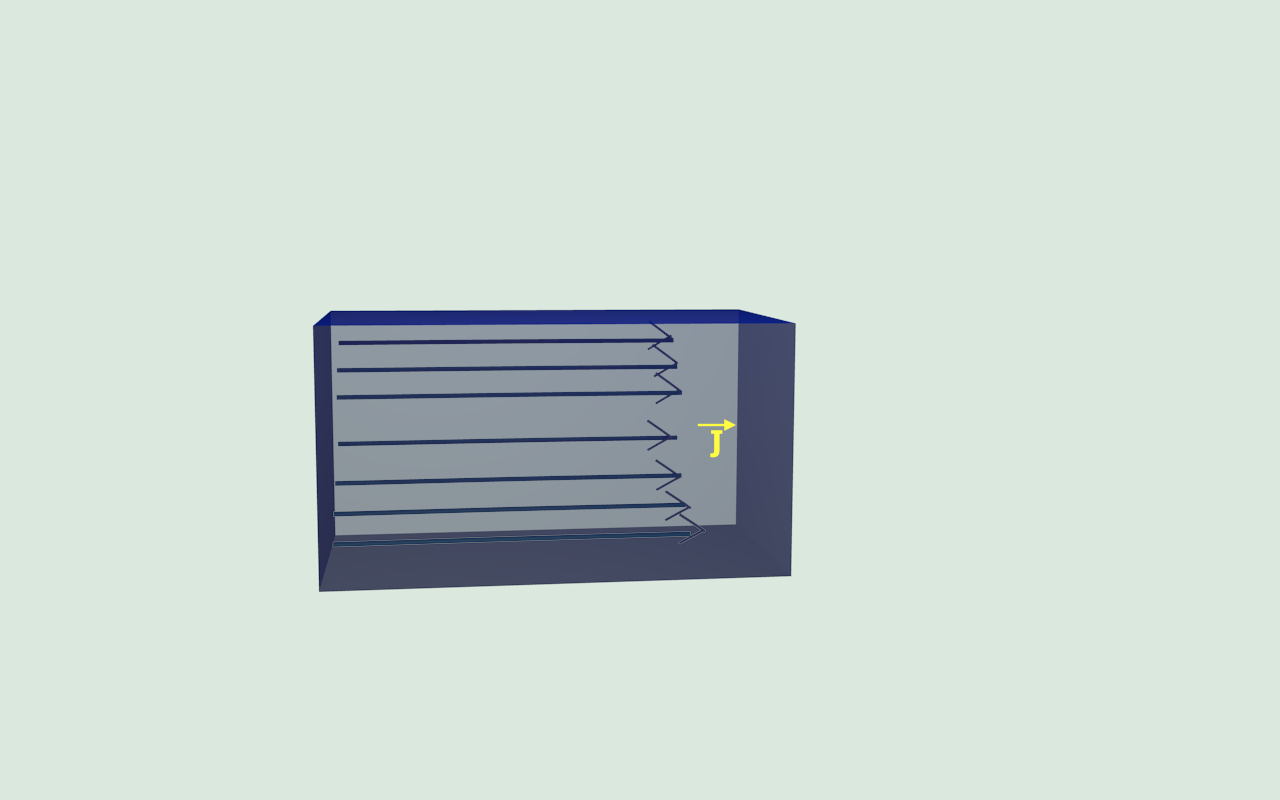
\includegraphics[height = 6cm, keepaspectratio]{graphes/blender_cuve_champvec.png}
		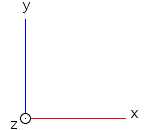
\includegraphics[height = 2cm, keepaspectratio]{graphes/axes.png}
		\caption{liquide faiblement ionisé soumis à un champ électrique $\vec{E}$}
%		\end{subfigure}
%		\begin{subfigure}[b]{0.3\textwidth}
		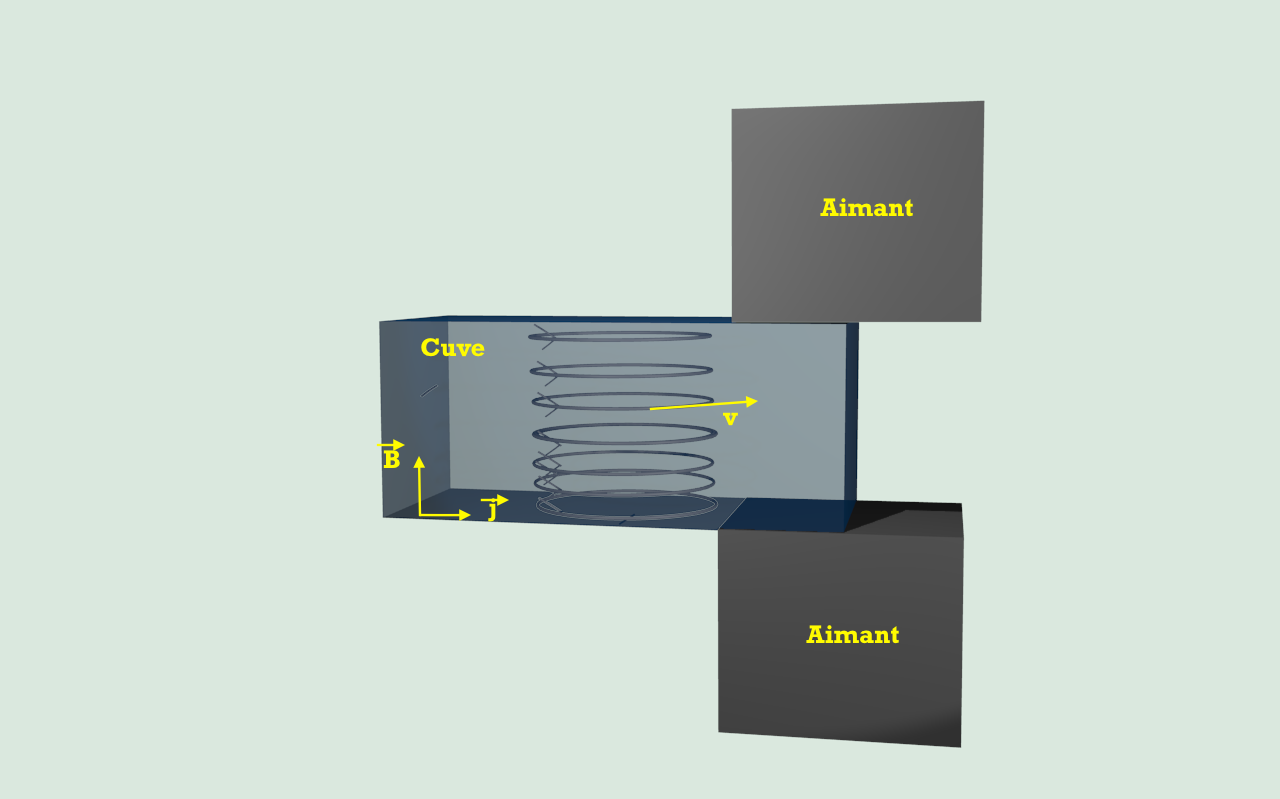
\includegraphics[height = 8cm, keepaspectratio]{graphes/blender_cuve_champvec2.png}
		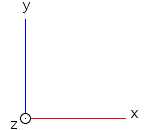
\includegraphics[height = 2cm, keepaspectratio]{graphes/axes.png}
		\caption{liquide faiblement ionisé soumis à un champ électrique et un champ magnétique $\vec{B}$}
%		\end{subfigure}
	\end{center}
\end{figure}
\subsection{dispositif expérimental} 



Expérimentalement, il est possible de réaliser cet écoulement à l’aide d’une distribution adéquate des forces. Pour cela, on utilise un système composé de parallélépipède, d’aimants permanents et d’électrodes. Le parallélépipède est un mélangeur dans lequel se trouve un liquide faiblement conducteur.
Afin de générer un tourbillon, on place deux aimants l’un en face de l’autre sur une moitié du parallélépipède pour créer un champ $\vec{B}$ vertical sur cette moitié. On place aussi deux électrodes sur les deux autres faces opposées du parallélépipède pour créer un courant uniforme de densité $\vec{j}$.
 
Afin de générer deux tourbillons, on place deux aimants l’un en face de l’autre sur le deuxième tiers du parallélépipède pour créer un champ B~ vertical sur le tiers au milieu.
On place aussi deux électrodes sur les faces opposées du parallélépipède pour créer un courant uniforme de densité $\vec{j}$.
Une force de Laplace est générée, due a` la difference de potentiel (P1 - P0) en présence d’un champ magnétique $\vec{B}$, deux tourbillons sont alors générés dans le parallélépipède
%Pour obtenir la situation de 3 tourbillon dans une cuve avec 2 parallèles er le dernier perpendiculaires aux 2 autres, nous allons utiliser un liquide faiblement conducteur soumis à un champ électrique est à des champs magnétiques pour créer les tourbillon : On place trois aimants pour générer les trois tourbillons créant ainsi un mouvement d'advection chaotique.


\begin{figure}[!h]
\begin{center}
%\centering
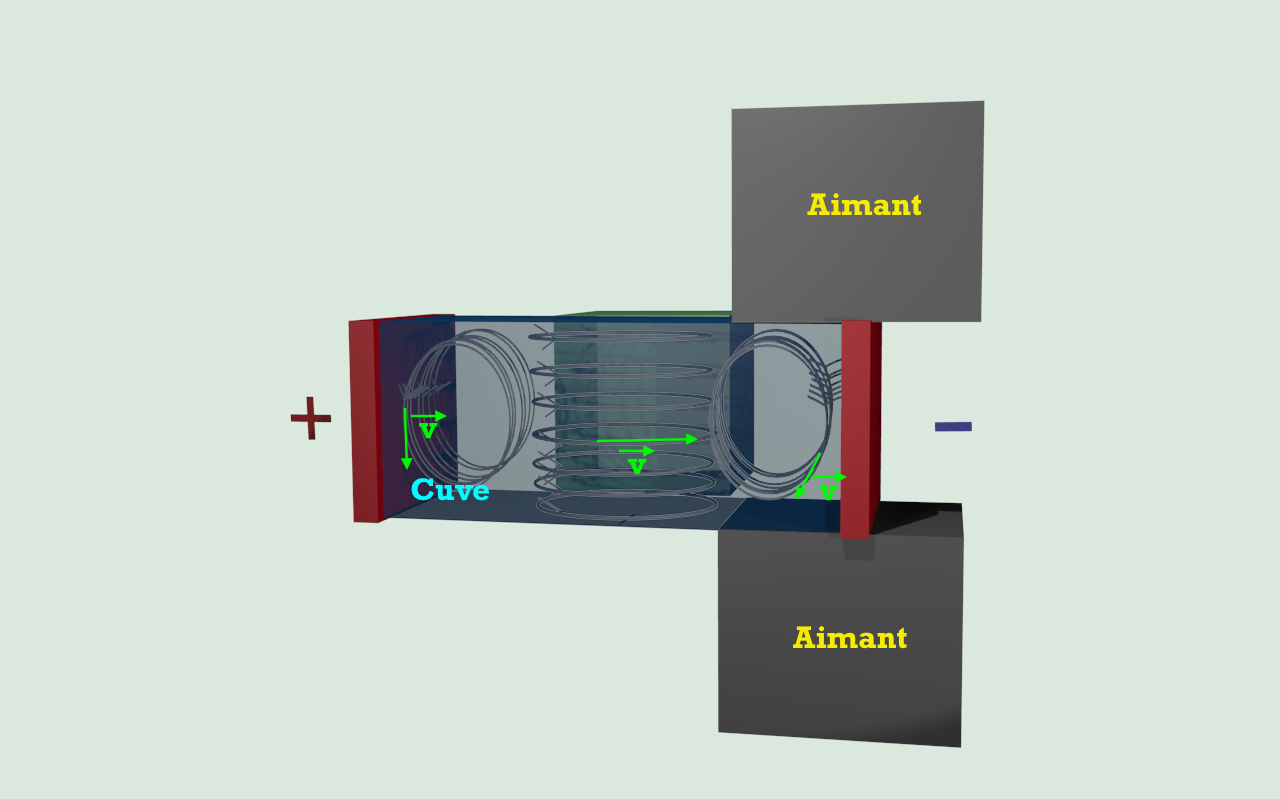
\includegraphics[height = 8cm, keepaspectratio]{graphes/blender_cuve_champvec3.png} 
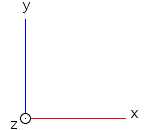
\includegraphics[height = 2cm, keepaspectratio]{graphes/axes.png}
\caption{advection chaotique avec trois tourbillons}
\end{center}
\end{figure}


\newpage
\subsection{hypothèses de modélisation}
Nous devons d'abord modéliser notre système , car dans les cas de système faisant intervenir des équations à dérivées partielles , la bonne définition du système est primordiale, avec notamment la prédominance des conditions aux limites dans la catégorie de problèmes que nous traitons. \\
Notre système sera modélisé par un fluide visqueux incompressible régi par les équations de Stokes qu’on verra dans le chapitre suivant. Les forces électromagnétiques seront aussi modélisées par des forces constantes dans une certaine région du domaine et générant ainsi les trois tourbillons souhaités. Nous allons nous intéresser tout d’abord aux équations du système.
%=========================================================================================================================================================
%												chapitre 2 equations de Navier_Stockes
%=========================================================================================================================================================
\newpage
\chapter{Équations de  Navier Stokes} 
D'après ce qui précéde, le fluide considéré suit les équations de Navier-Stokes dont nous allons nous servir pour modéliser le mouvement.
Nous supposons que nous avons à notre disposition deux aimants, qui sont perpendiculaires sur les côtés de la cuve, l'un produit un champ $B_1$, l'autre produit un champ $B_2$
\begin{figure}[!h]
\begin{center}
\centering
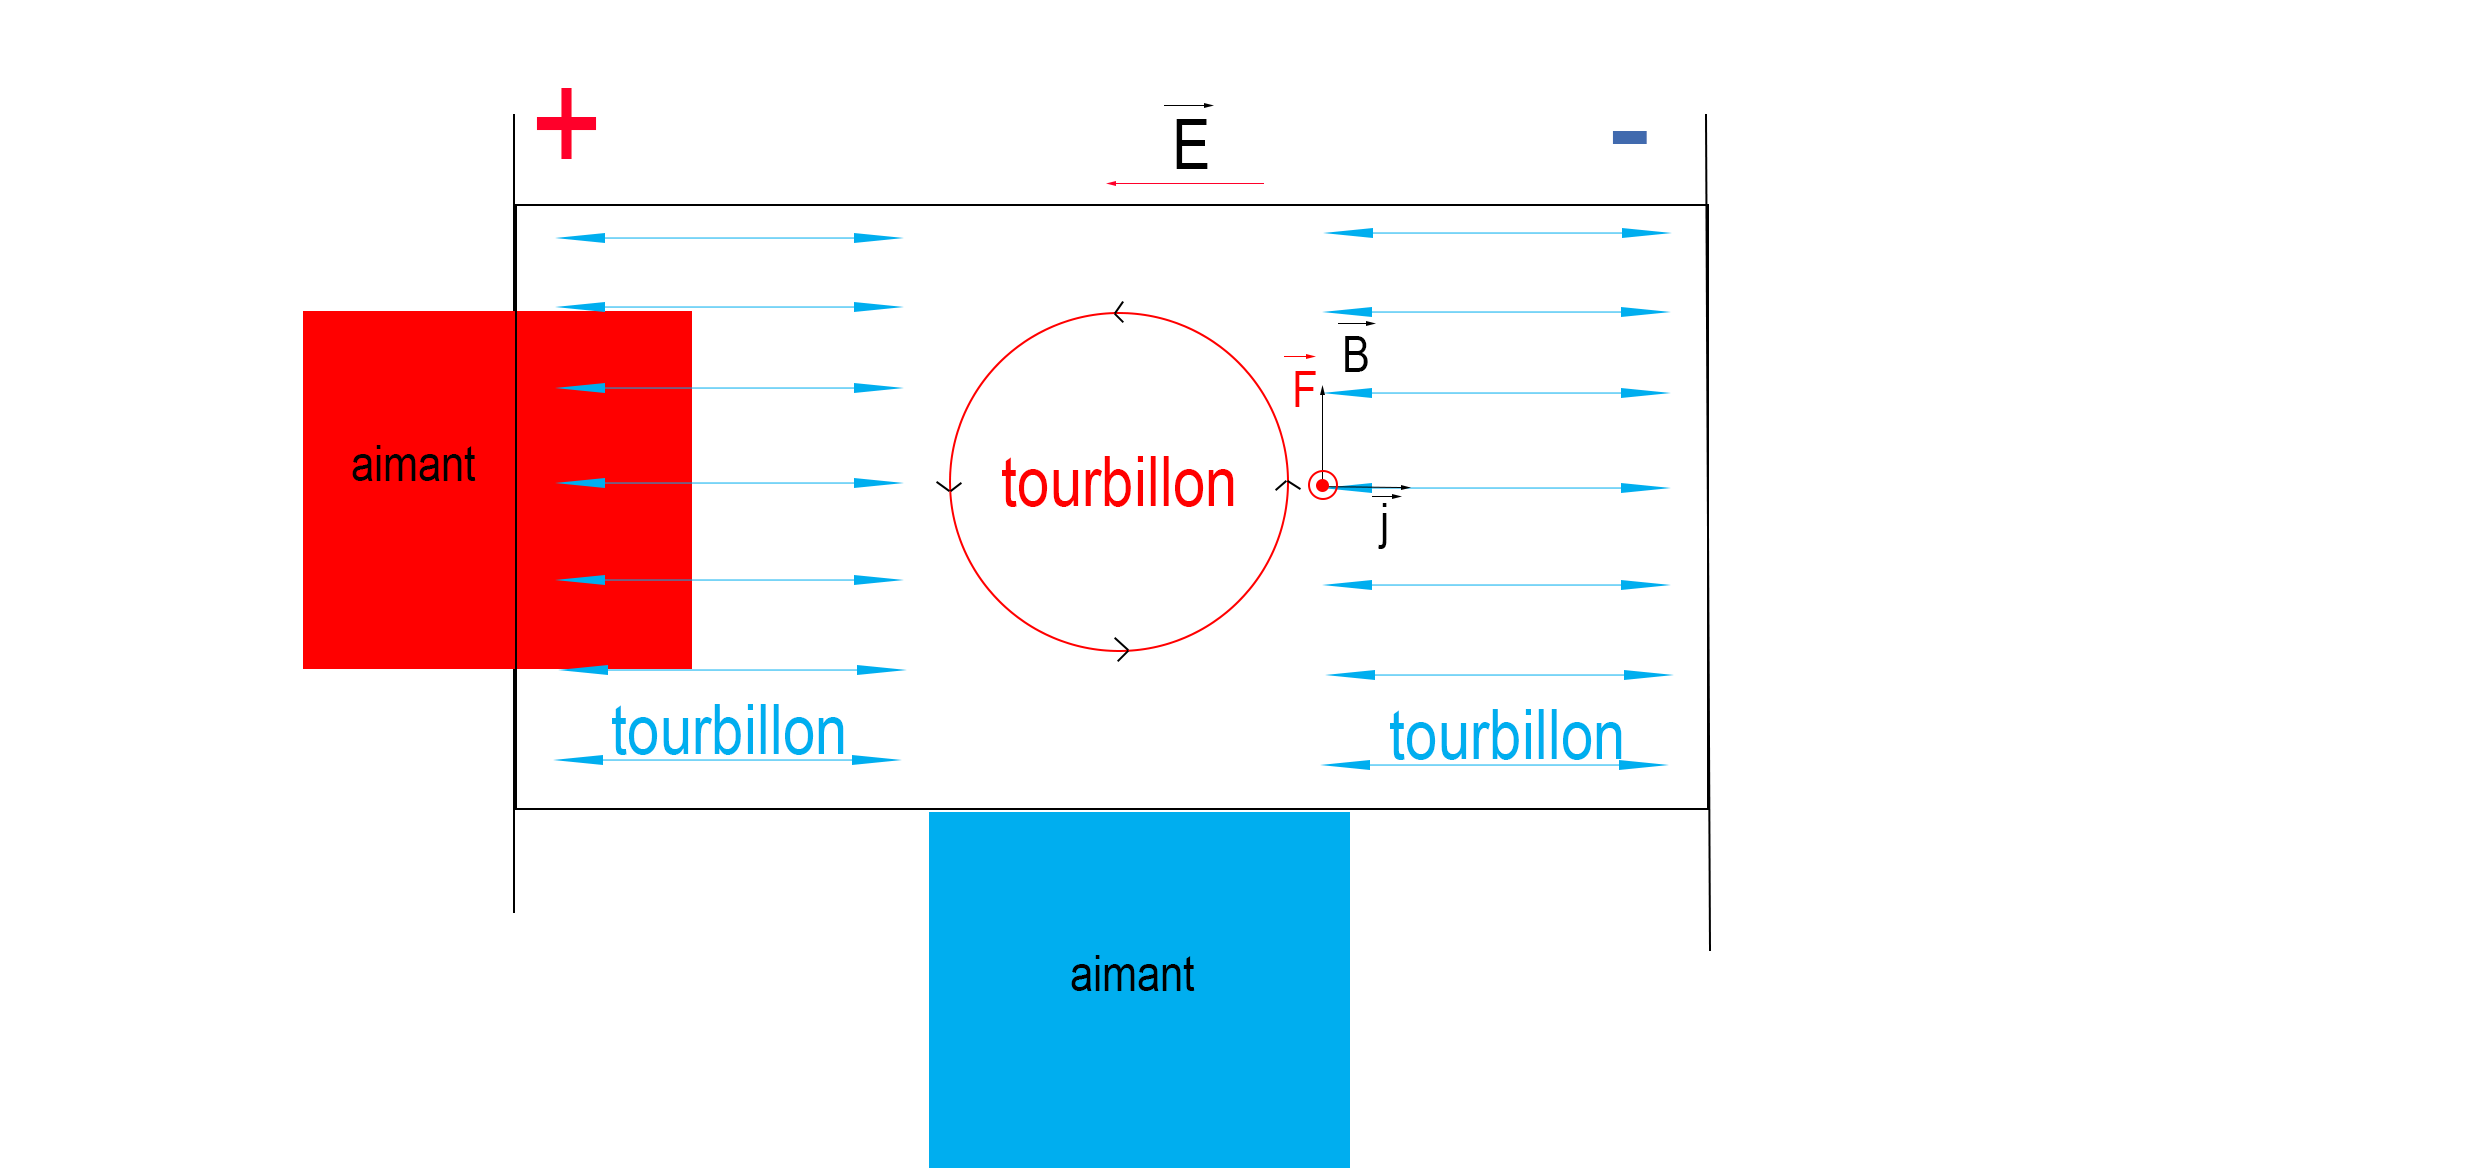
\includegraphics[height = 6cm, keepaspectratio]{graphes/cuveaimant4.png} 
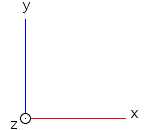
\includegraphics[height = 2cm, keepaspectratio]{graphes/axes.png}
\caption{advection chaotique avec trois tourbillons}
\end{center}
\end{figure}
\newpage
le premier aimant va produire un tourbillon dans le fluide, le deuxième va produire deux tourbillons parallèles, qui sont orthogonaux au premier tourbillon  : 
\[
	B_1 = 
	\begin{pmatrix}
   		B_{1,x}\\
  		 B _{1,y}\\
  		 0
	\end{pmatrix} \
	\text{et} \
	B_2 = \begin{pmatrix}
  			 0\\
   			B _{2,y}\\
   			B_{2,z}
			\end{pmatrix}
\]
\\

Ainsi on peut calculer la force magnétique \\%
\[
	\vec{f_1}=j_0\vec{e}_{x}
	\wedge\begin{pmatrix}
   		B_{1,x}\\
   		B _{1,y}\\
   		0
\end{pmatrix}=
j_0\times \begin{pmatrix}
  			0\\
   			0\\
    		B_{1,y}
			\end{pmatrix} 
\]
\\%
 et 
\[
	\vec{f_2}=j_0\vec{e}_x\wedge\begin{pmatrix}
   					0\\
   					B _{2,y}\\
   					B_{2,z}
					\end{pmatrix}
	=
	j_0\times \begin{pmatrix}
   				0\\
   				-B _{2,z}\\
   				B_{2,y}
		\end{pmatrix} 
\]
\\%

On peut donc écrire pour la force magnétique totale $\vec{f}$
\[
	\vec{f}=\vec{f_1}+\vec{f_2}=\begin{pmatrix}
   B_1,x\\
   B _1,y\\
   0
\end{pmatrix} 
\]
\\%

%===================================================== Equations de Stokes ================================================================================
\subsection{Équations de Stokes}

Le liquide est un conducteur placé dans un champ magnétique et parcouru par un courant uniforme $\vec{J_0}$. Une force de Laplace $\vec{f_l}$ est alors créée. La densité volumique de cette force est donnée par :
\[
	\vec{f_l}=\vec{j_0}\land\vec{B}=j_0\times M_0\times \vec{j}\wedge \vec{B^*}
\]
%mec est-ce qu'on a droit aux docs demain ?

\[
	 \vec{B^*} =\frac{\vec{B}}{M_0}, 
	\ \text{et} \ j_0=\frac{\Delta P}{L}\sigma
\]

%																	ajouter figure graphe
\begin{figure}[h]
\begin{center}
%&\includegraphics[height =4 cm, keepaspectratio]{graphes/graphe_forces_laplace} 
\caption{}
\label{figure 1}
\end{center}
\end{figure}
Avec :
\[-
\begin{aligned}
&-\sigma : \text{la conductivité du fluide }
\\%
&\text{-L: la longueur de base de la cuve}
\end{aligned}
\]
\normalsize 
Afin de pouvoir trouver l'équation de la trajectoire d’un point donné, on cherche tout d’abord à trouver la vitesse dans l'écoulement du fluide contenu dans un domaine $\Omega$.
\\A partir des équations de Navier-Stokes incompressibles, on détermine simultanément la vitesse  $V$ et la pression $P$. 
\\
\\
On émet les hypothèses suivantes :
\\
Dans un premier temps, nous pouvons négliger les forces d’inertie du fluide comme on a un faible nombre de Reynolds.
Le fluide visqueux est en mouvement le long d’une paroi solide fixe d’où une vitesse nulle sur le bord car 
$\vec{V_{\partial\Omega}}=\vec{V_{\text{paroi}}}=\vec{0}$
\\	
Finalement, on se place en régime stationnaire.
\begin{equation*}
  \left\{
    \begin{aligned}
      &\vec{0}=-\vec{\bigtriangledown}P +\mu\vec{\Delta}V +\vec{f}\;\text{dans }\Omega \\
      &\text{div}(\vec{V})=0\;\text{dans }\Omega \\     
      &\vec{V}=\vec{0}\;\text{sur }\partial\Omega
    \end{aligned}
  \right.
\end{equation*}

%==================================================== Adimensionnement de l'équation de Stokes ============================================================

\subsection{Adimensionnement de l'équation de Stokes}

\normalsize Afin de résoudre un seul système indépendamment des constantes, on adimensionne l'équation de Stokes. Le régime stationnaire sera pris en compte après adimensionnement.
\\%
Posons :
\begin{equation*}
\vec{V'}(x,t)=\frac{\vec{V}(x,t)}{V_0}\;;\vec{x'}=\frac{\vec{x}}{L_0}\; ; \vec{f'}(\vec{x'})=\frac{\vec{f}(\vec{x})}{j_0M_0}\;;P'=\frac{P}{P_0}\; ;t'=\frac{t}{\frac{L_0^2}{\mu}}\;
\end{equation*}
En injectant dans l'équation de Stokes d'évolution :
\begin{equation*}
  \left\{
    \begin{aligned}
    \rho\frac{\partial \vec{V}}{\partial t}=-\vec{\bigtriangledown} P + \mu \vec{\Delta}\vec{V}+\vec{f}
        \end{aligned}
  \right.
\end{equation*}
il en résulte :
\begin{equation*}
  \left\{
    \begin{aligned}
    \frac{\partial \vec{V'}}{\partial t}=-\frac{L_0 P_0}{\rho \mu V_0}\vec{\bigtriangledown} P '+  \vec{\Delta}\vec{V'}+\frac{L_0^2j_0M_0}{\mu V_0}\vec{f'}
        \end{aligned}
  \right.
\end{equation*}
On adimensionne par rapport à $V_0$ et $P_0$ de sorte que $\frac{L_0 P_0}{\rho \mu V_0}=1$ et $ \frac{L_0^2j _0M_0}{\mu V_0}=1$, le régime stationnaire étant établi:
\[
      \vec{0}=-\vec{\bigtriangledown}P' +\vec{\Delta}V' +\vec{f'}\;\text{dans }\Omega 
\]

%========================================================= Formulation variationnelle =====================================================================
\subsection{Formulation variationnelle}

Afin d'obtenir la formulation variationnelle de l'équation de Stokes, on passe dans l'espace des distribution de sorte que pour toute fonctions test $\varphi$ on a 
\[
	\int_\Omega\vec{\bigtriangledown}P'\times \vec \varphi=\int_\Omega-\mu\vec{\Delta}V'\times \vec \varphi +\int_\Omega\vec{f'}\times \vec \varphi 
\]
En appliquant la formule de Green, on obtient :

\[
\forall \varphi \in D(\Omega) \quad  \int_\Omega\vec{\bigtriangledown}P'. \vec \varphi + \int_{\Omega}\bigtriangledown V'. \bigtriangledown \varphi = \int_\Omega\vec{f'}. \vec \varphi
\]
Comme précédemment nous nous plaçons dans l'espace $V_{h}$ d'approximation polynomiale de degrés 1.
Nous pouvons ainsi décomposer les champs de pression $P'$, la vitesse $V'$ et la force $\vec{f'}$ dans la base des $(\varphi_{i})$:

\begin{equation*}
  \left\{
    \begin{aligned}
 &V '= \sum_{i=1}^{N_{h}}{\ V_{i}\varphi_{i}} \text{ \ \ où } V_{i} = V(P_{i}),\  i= 1,2,...,N_{h}\\
 &P '= \sum_{i=1}^{N_{h}}{\ P_{i}\varphi_{i}} \text{ \ \ où } P_{i} = P(P_{i}),\  i= 1,2,...,N_{h}\\
 &f' = \sum_{i=1}^{N_{h}}{\ f_{i}\varphi_{i}} \text{ \ \ où } f_{i} = f(P_{i}),\  i= 1,2,...,N_{h}\\
\end{aligned}
  \right.
\end{equation*}$ $ \\ 
On prend $\varphi\ =\ \varphi_{i}$ un vecteur de la base
\begin{equation*}
  \left\{
    \begin{aligned}
	&\int_{\Omega}\bigtriangledown V_{h}.\bigtriangledown \varphi\ 
	=\ 
	\sum_{i, j \in [1, N_{h}]^{2}} \int_{\Omega}V_{i}\bigtriangledown\varphi_{i}. \bigtriangledown\varphi_{j} 
	= 
	\sum_{i,j \in [1, N_{h}]^{2}} A_{ij} V_{i}\\
	&\int_{\Omega}\bigtriangledown P_{h}.\varphi\ 
	=\ 
	\sum_{i, j \in [1, N_{h}]^{2}} \int_{\Omega}P_{i}\bigtriangledown\varphi_{i}. \varphi_{j} 
	= 
	\sum_{i,j \in [1, N_{h}]^{2}}C_{ij} u_{i}\\
	&\int_{\Omega} f. \varphi\ 
	=\ 
	\sum_{i, j \in [1, N_{h}]^{2}} \int_{\Omega}f_{i}\varphi_{i}. \varphi_{j} 
	= 
	\sum_{i,j \in [1, N_{h}]^{2}} M_{ij} f_{i}\end{aligned}
  \right.
\end{equation*}
On peut donc écrire la formulation variationnelle sous la forme d'un problème linéaire:
\begin{equation*}
  \left\{
    \begin{aligned}
	&-A\times V + C \times P = M	\times f \ \text{sur} \ \Omega\\
	& C*V = 0 \ \text{sur} \  \partial\Omega\\
	\end{aligned}
  \right.
\end{equation*}


La linéarité de l'équation nous permet d'appliquer le principe de supperposition est donc de décomposer la résolution du problème en deux résolutions : une pour chaque terme source et ensuite de les sommer.
Pour cela, nous allons chercher à calculer le terme source dans la suite, c'est à dire le champ magnétique.

%=====================================================================================================================================
%												CHAPITRE 1 CALCUL DU CHAMP MAGNETIQUE
%==========================================================================================================================================================
\newpage
\chapter{Modélisation du champ Magnétique de l'aimant}

Nous cherchons dans cette partie à déterminer une approximation du champ magnétique $\vec{B}(x,y,z)$ induit par un aimant (Figure 1). L'objectif sera d'abord de déterminer le champ magnétique dans un milieu quelconque, pour ensuite exploiter ces résultats pour les employer dans la résolution numérique de Navier Stokes. 
\begin{figure}[h]
\begin{center}
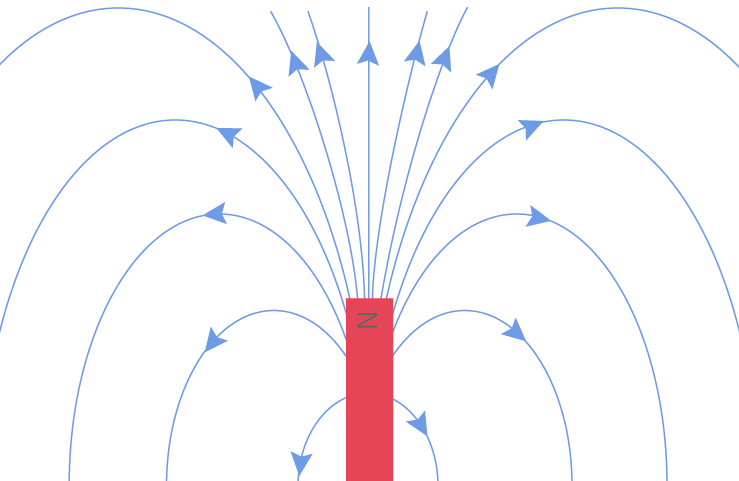
\includegraphics[height =4 cm, keepaspectratio]{graphes/champ_aimant1.png} %on affiche figure aimant
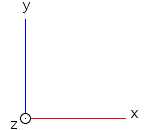
\includegraphics[height = 2cm, keepaspectratio]{graphes/axes.png}
\caption{champ magnétique d'un aimant coupe 2D}
\label{figure 1}
\end{center}
\end{figure}
\newline
\begin{figure}[!h]
\begin{center}
\centering
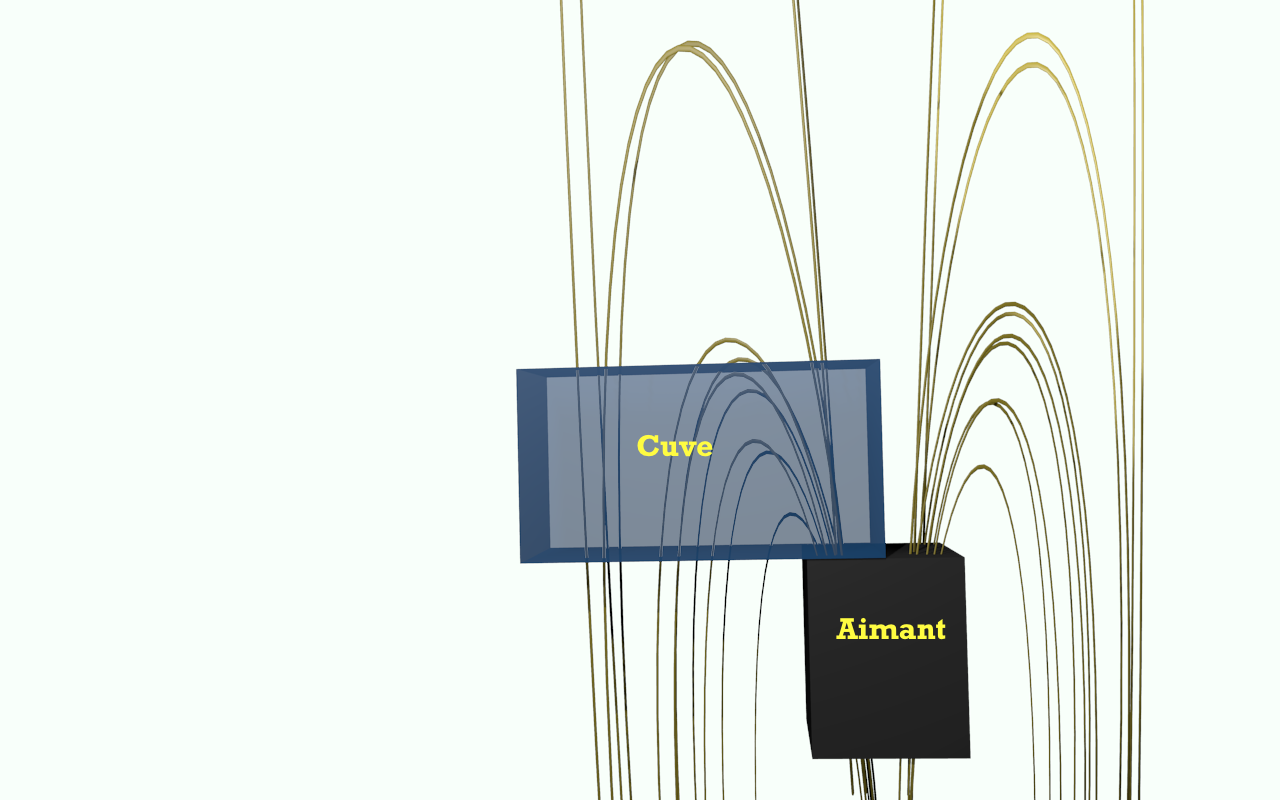
\includegraphics[height = 8cm, keepaspectratio]{graphes/blender_cuve_mag2.png} 
\caption{advection chaotique avec trois tourbillons}
\end{center}
\end{figure}
On suppose que l'aimant à une longueur suffisante selon $\vec{z}$ pour être considéré comme infini selon $\vec{z}$.
On en déduit donc par le principe de Curie que le champ magnétique est invariant par translation selon $\vec{z}$. 
Ainsi \[\vec{B}(x,y,z) = \vec{B}(x,y)\]

%============================================== Mise en forme du probleme =================================================================================
\section{Mise en forme du problème}

Nous allons rechercher une solution du champ magnétique dans le domaine de résolution $\Omega$ (figure 2), $\Omega \subset R^{2}$. \\
\begin{figure}[h]
\begin{center}
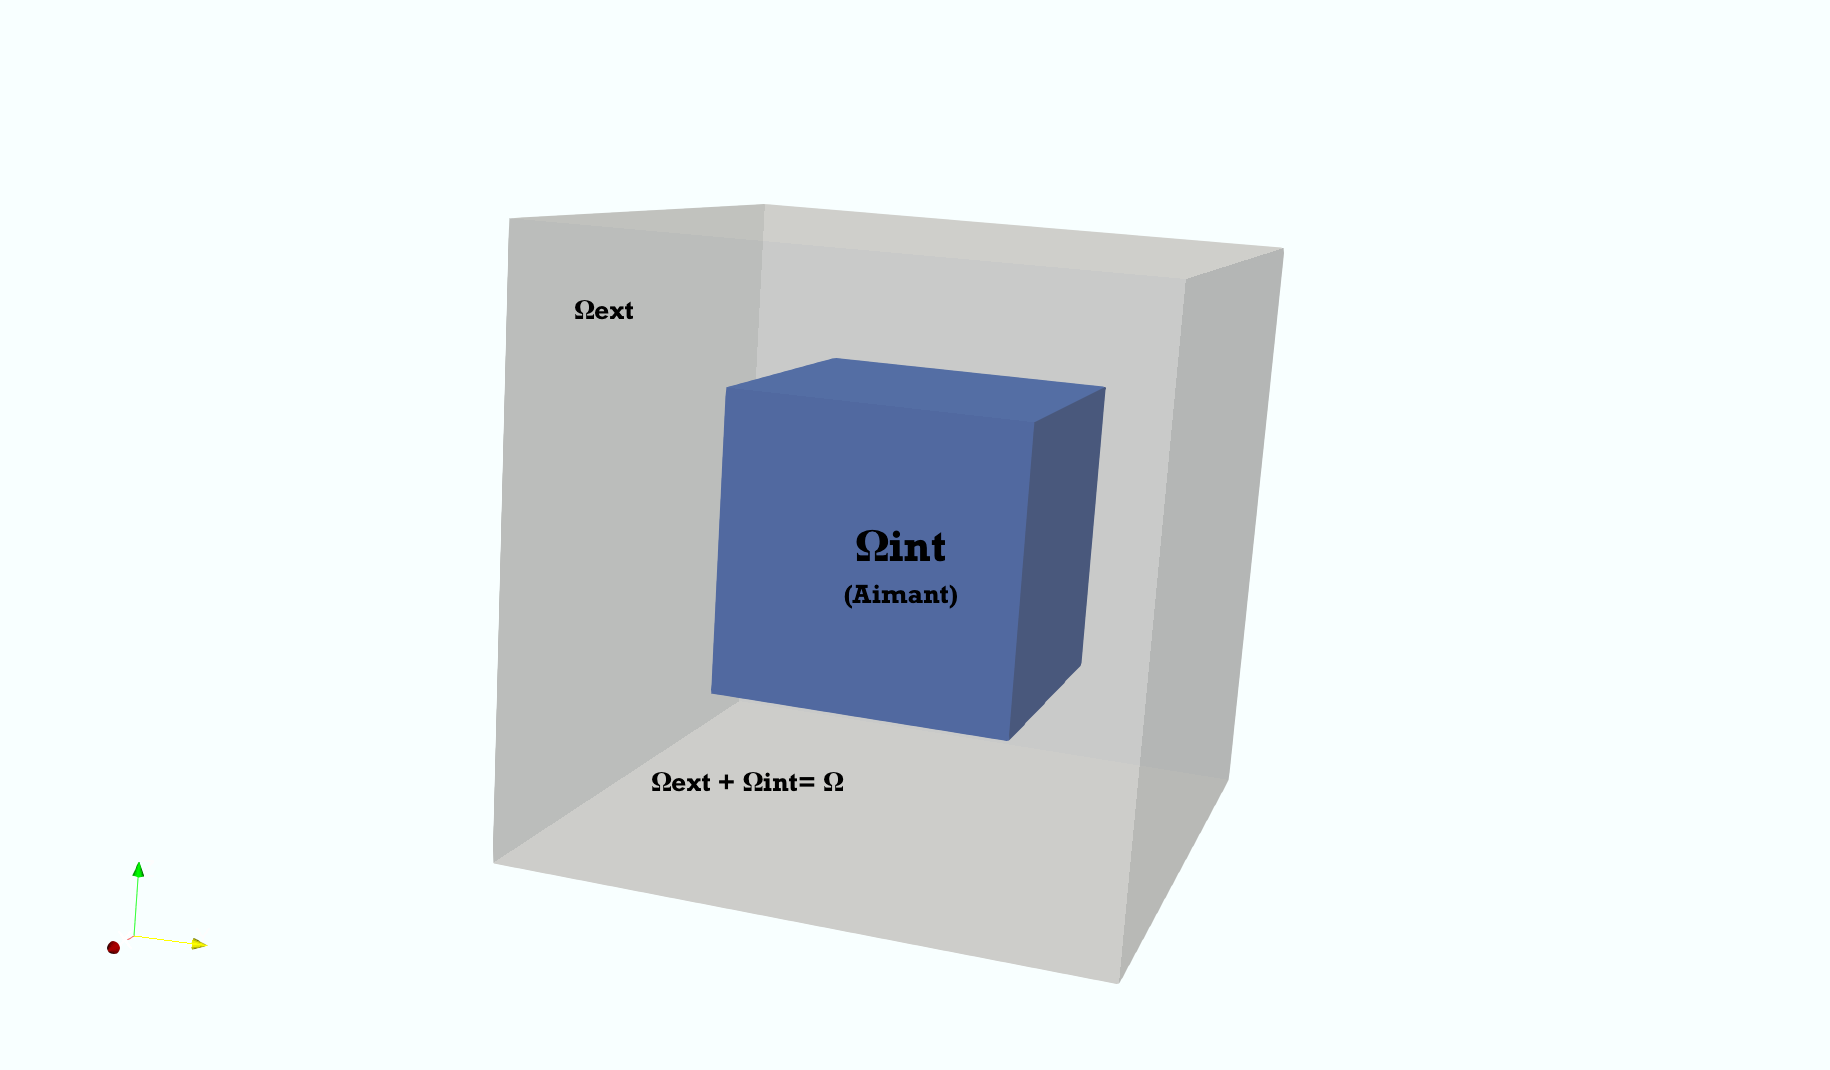
\includegraphics[height = 8cm, keepaspectratio]{graphes/Espacedetravail.png} 
\caption{domaines de résolution du problème}
\label{figure 2}
\end{center}
\end{figure}
On définit $\Omega_{int}$ le domaine de l'aimant, et $\Omega_{e}$ le domaine extérieur à l'aimant. 
\[\Omega_{e} = \Omega_{int} - \Omega\]

\newpage
On se place dans le régime stationnaire comme il n'y a pas de mouvements de l'aimant. \\
Le champ d'induction magnétique $\vec{B}$ est la somme du champs magnétique $\vec{H}$.

\[\vec{B}=\mu _{0}(\vec{H}+\vec{M})\]
$\mu _{0}$ est la perméabilité magnétique du vide. \\
L'aimantation $\vec{M}$ est nulle en dehors de l'aimant.
 
\[ 
\left\{
\begin{array}{ccc}
\begin{aligned}
	\vec{M} &= \vec{0} \  \text{dans} \ \Omega_{e} \\ 
	\vec{M} &= \vec{M_{0}} = \text{constante}  \ \text{dans}  \  \Omega_{\text{int}}
\end{aligned}
\end{array}
\right.
\]

Pour trouver le champ magnétique, on appliquer les équations fondamentales de la magnétostatique. L'équation de Maxwell nous donne 
\[
	\left\{
	\begin{array}{ccc}
	\begin{aligned}
		\Rot{\vec{H}} &= \vec {0} \\
		\Div{\vec{B}} &= 0
	\end{aligned}
	\end{array}
	\right.
\]

Le domaine étant simplement connexe, $\vec{H}$ dérive d'un potentiel $u$	.
\[
	\left\{
	\begin{array}{ccc}		
	\begin{aligned}
		\vec{H} &= \Grad{\vec{u}} \\
		\vec{B} &= \mu_{0}\times(\vec{\Grad{u}}+\vec{M})
	\end{aligned}
	\end{array}
	\right.
\]

Au sens des distributions pour toute fonction $\varphi\ $  dans $D(\Omega)$	
\[<\Div\vec{B},\varphi> \ = \ <-\vec{B},\vec{\Grad{\varphi}}>\]
On suppose $\vec{B} \in L^{3}_{1}(\Omega)$
\[<\Div\vec{B},\varphi> \ = \  -\int_{\Omega}\vec{B}. \vec{\Grad{\varphi}}\]
\[<\Div\vec{B},\varphi> \ = \ -\int_{\Omega}\mu_{0}(\vec{\Grad{u}}+\vec{M}) .{\Grad{\varphi}} = 0\]
Ainsi
\[\int_{\Omega}(\vec{\Grad{u}}+\vec{M}) . \vec{\Grad{\varphi}} = 0\]
Et comme $\vec{M}$ est nul en dehors du domaine $\Omega_{\text{int}}$ de l'aimant, on obtient (1)

On reconnait un problème de Dirichlet homogène qui admet une unique solution dans $H_{0}^{1}(\Omega)$ d'après le théorème de Lax-Migram.
\begin{equation}
\label{E}
\forall \varphi\ \in \Omega, \ \int_{\Omega}\bigtriangledown u .\bigtriangledown{\varphi} = -\vec{M_{0}}. \int_{\Omega_{int}}\bigtriangledown\varphi
\end{equation}

Adimensionnons (1)				:
\[
	\forall \varphi\  \in \Omega,\  \frac{1}{|\vec{M}_{0}|}\int_{\Omega}\bigtriangledown u.\bigtriangledown \varphi
	= -\vec{e}_{y}.\int_{\Omega_{int}}\bigtriangledown \varphi
\]
On prend pour la suite \[U =  \frac{u}{|\vec{M}_{0}|}  \] ce qui nous donne \[\vec{H^*} =\frac{\vec{H}}{M_0} \]
On établit ainsi \label{A}

\begin{equation}
\boxed{
\label{A}
	\forall \varphi\  \in \Omega,\ \int_{\Omega}\bigtriangledown U.\bigtriangledown \varphi
	=- \vec{e}_{y}.\int_{\Omega_{int}}\bigtriangledown \varphi}
\end{equation}
\\

\section{Méthode des éléments finis}

\subsection{Le maillage}
On recherche une solution approchée de l'équation numériquement en passant de l'espace continu à un espace discret. \\
\\
On utilise la méthode des éléments finis en recherchant une solution dans l'espace 
$V_{h} = \{u \ | \ u \in P^{1}(\Omega^{2}), u \in H^{1}_{0}(R^{2})\}$. \\
\\
On introduit une triangulation $T_{h}$ en subdivisant $\overline{\Omega}$, \\ de bord $\Gamma \ = \ \partial\Omega$. 
\newpage
Cette triangulation vérifie les propriétés suivantes :
\\
\begin{itemize}
  \item l’intersection de deux triangles de $T_{h}$ doit être réduite à un sommet commun,\\ à une arête commune et entière ou à l'ensemble vide
  \item l’aire des triangles ne doit pas être nulle
  \item tous les coins du bord $\Gamma$ sont des sommets de triangles de $T_{h}$
\end{itemize}

Le maillage ainsi construit est tel que
\[
\overline{\Omega} \ = \ \bigcup_{K \in T_{h}} K 
\]
\begin{figure}[h]
\begin{center}
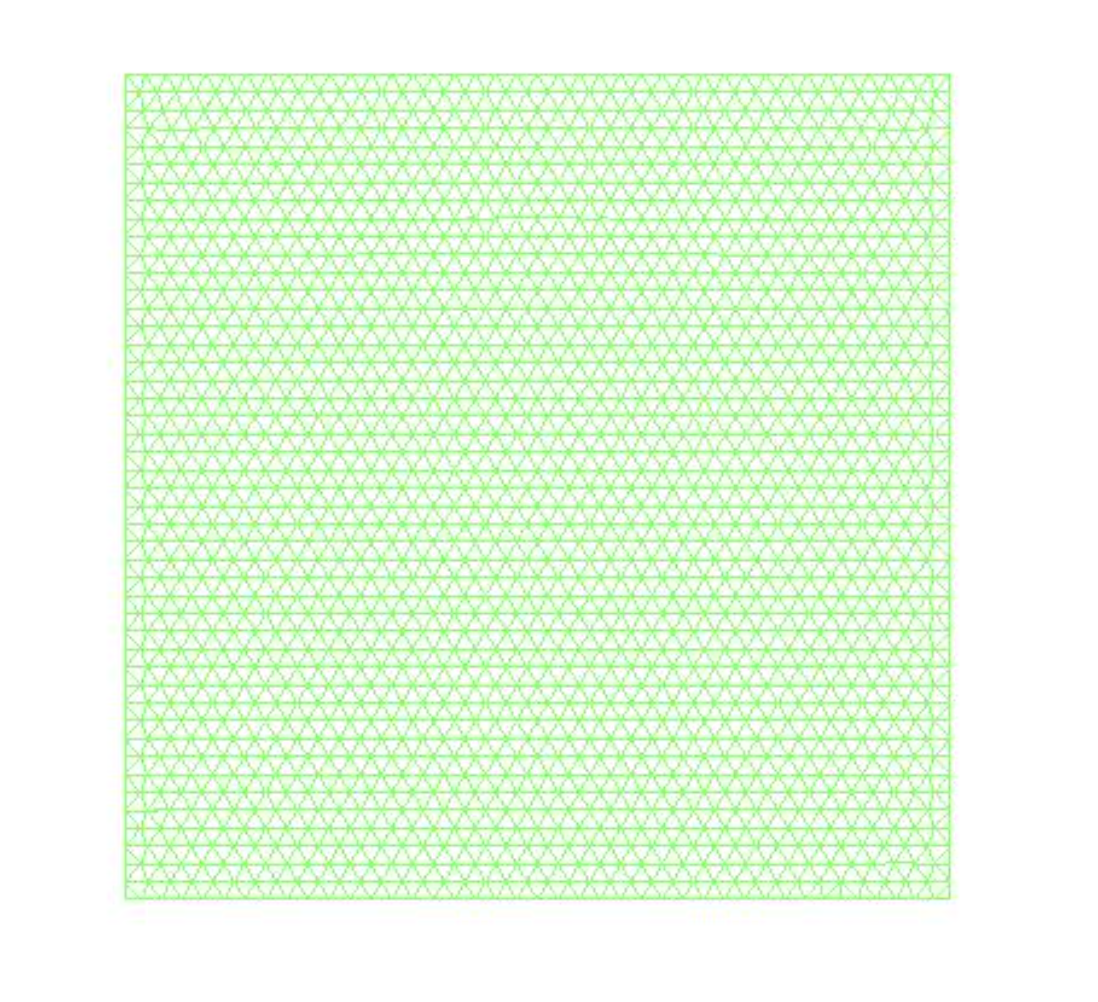
\includegraphics[height = 8cm, keepaspectratio]{graphes/Maillage_initial.png} 
\caption{\label{figure 3 } maillage effectué sur matlab à l'aide de mesh2D d'un carré 1$\times$1.05 avec un pas constant h = 0.1}
\end{center}
\end{figure}

On note que le maillage est caractérisé par la longueur de la plus petite arrête $h_{min}$ telle que 
\[
h_{min} \ = \ \min_{K \in T_{h}} h_{K}
\]
$h_{min}$ va notamment déterminer l'erreur entre la solution continue et la solution discrète.
§

On choisit une base de $V_{h}$, on prend la famille des fonctions de base  \\ $\varphi_{1}, \varphi_{2}, ..., \varphi_{N_{h}}$  telles qu'elles valent 1 en un sommet d’un triangle, et 0 pour tous les autres sommets. On note $P_{1},P_{2}, ..., P_{N_{h}}$ les sommets des triangles du maillage.
Les fonctions de base sont donc définies ainsi :
\[
\forall i,j \in [1, N_{h}]^{2} \ \varphi_{i} \in L^{2}(\Omega),\ \varphi_{i}(P_{j}) \ = \ \delta_{ij} \ \
\varphi_{i} \ = \ 0 \ sur \ \Gamma \]
Le support de $ \varphi_{i}$ est la réunion de tous les triangles ayant pour sommet $P_{i}$.\\
On vérifie que la famille ($\varphi_{1}, \varphi_{2}, ..., \varphi_{N_{h}}$) est une base de $V_{h}$.
Ainsi toute fonction g dans $V_{h}$ peut s'écrire comme une combinaisons linéaire des $\varphi_{i}$
\[
g = \sum_{i=1}^{N_{h}}{\ g_{i}\varphi_{i}} \text{ \ \ où } g_{i} = g(P_{i}),\  i= 1,2,...,N_{h}
\]
 
\subsection{Mise en équation}


Réécrivons (1.2) dans $V_{h}$ : 

\[
	\forall \varphi \in V_{h} , \ \int_{\Omega}\bigtriangledown u_{h}. \bigtriangledown \varphi = -\vec{M_{0}}. \int_{\Omega_{int}}\bigtriangledown \varphi
\]
Nous pouvons écrire $u_{h} = \sum_{i=1}^{N_{h}}{\ U_{i}\varphi_{i}} \text{ \ \ où } U_{i} = U(P_{i}),\  i= 1,2,...,N_{h}$ \\ et choisir $\varphi\ =\ \varphi_{i}$
ainsi
\[
	\int_{\Omega}\bigtriangledown u_{h}.\bigtriangledown \varphi\ 
	=\ 
	\sum_{i, j \in [1, N_{h}]^{2}} \int_{\Omega}u_{i}\bigtriangledown\varphi_{i}. \bigtriangledown\varphi_{j} 
	= 
	\sum_{i,j \in [1, N_{h}]^{2}} A_{ij} u_{i}
\]
avec A la matrice $N_{h} \times N_{h}$ de coefficients
\[
A_{ij}  = \int_{\Omega}\bigtriangledown\varphi_{i}.\bigtriangledown\varphi_{j}
\]
et si on introduit le vecteur $\vec{f}$ de composantes $f_{1},\ f_{2},..., f_{N_{h}}$ définies par
\[
f_{j} =  -\vec{e_{y}}.\int_{\Omega} \bigtriangledown\varphi_{j}
\]
Alors l'équation (2) revient de manière équivalente à résoudre le système linéaire 
\[
	A \times U =F
\]
 avec 
\[
U = 
\begin{pmatrix}
   u_{1} \\
   u_{2} \\
   \vdots \\
   u_{N_{h}}
\end{pmatrix}
\ \ F = 
\begin{pmatrix}
   f_{1} \\
   f_{2} \\
   \vdots \\
   f_{N_{h}}
\end{pmatrix}
\quad
A_{ij}  = \int_{\Omega}\bigtriangledown \varphi_{i}. \bigtriangledown \varphi_{j}
\]
On appelle A la matrice de rigidité.  \\

%============================================= passage element de reference ==============================================================================
\newpage
\subsection{Passage à un élément de référence}
Pour les calculs on utilise un maillage référence  normalisé $\hat{T}$. On passe du triangle $\Hat{T}$ à $T$ à l'aide de la transformation $F$. 
\begin{figure}[h!]
\begin{center}
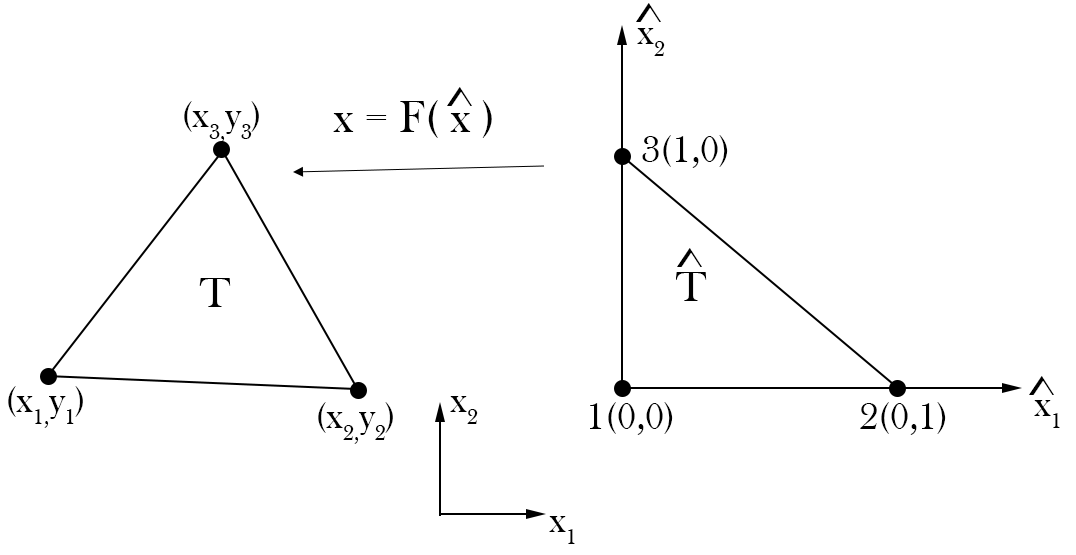
\includegraphics[height = 6cm, keepaspectratio]{graphes/transformation_de_maillage.png} 
\caption{\label{figure 4 } passage à un maillage de référence}
\end{center}
\end{figure}
On a pour le calcul du gradient de $\varphi_{i}$
\[ \bigtriangledown_{\hat{x}} \hat{\varphi} = (J)^{T} \bigtriangledown_{x} \varphi  \]
où J est la matrice Jacobienne de la transformation.
Calculons la matrice Jacobienne qui va dépendre des coordonnées $(x_{i},y_{i})$ des sommets pour chaque triangle.
\[
x = \begin{pmatrix}
   x_{1} \\
   x_{2} 
\end{pmatrix}
= \begin{pmatrix}
   F_{1}(\hat{x}) \\
   F_{2}(\hat{x}) 
\end{pmatrix}
= \begin{pmatrix}
   \hat{x}_{1} \\
   \hat{x}_{2} 
\end{pmatrix}
= J \times \hat{x} + C
\]
On obtient ainsi à l'aide d'un changement de variable le calcul de la matrice de rigidité (voir annexe A) : 
\[
\boxed{
\begin{aligned}
A_{ij} = 
	\iint_{\Omega}\bigtriangledown_{x}{\varphi_{i}} \bigtriangledown_{x}{\varphi_{j}} &= 
	\sum_{T \in \text{Supp}(\varphi_{i})\times \text{Supp}(\varphi_{j})}	
	\frac{\text{aire}(T)^{2}}{4}
	\begin{pmatrix}
   		y_{3}-y_{1} &  	x_{1}-x_{3}\\
   		y_{1}-y_{2} &  x_{2}-x_{1}
	\end{pmatrix}
	^{2}
	\bigtriangledown_{\hat{x}} \hat{\varphi_{i}}
	\bigtriangledown_{\hat{x}} \hat{\varphi_{j}}
\end{aligned}}
\]
\\
\\
Calculons à présent le terme source $f_{j} =  -\vec{e_{y}}.\int_{\Omega} \bigtriangledown\varphi_{j}$.
\\
\\
D'après Green-Ostrogradsky
\[
	\iint_{\Omega}\bigtriangledown_{x}{\varphi_{i}} =\ 
	\int_{\partial\Omega_{\text{int}}}\varphi_{i}.\vec{\text{n}} \ \partial s
\]

Ainsi	
\[
	\begin{aligned}
		\int_{\partial\Omega_{\text{int}}}\varphi_{i}.\vec{\text{n}}\ \partial s &= 
		\sum_{e \in \partial\Omega_{\text{int}}}\ \int_{e}\varphi_{i}.\vec{\text{n}}_{e}\ \partial s \\ &=  
		\sum_{e \in \partial\text{supp}(\varphi_{i})}\ \int_{e}\varphi_{i}.\vec{\text{n}}_{e}\ \partial s
	\end{aligned}
\]
où $\vec{\text{n}}_{e}$ est le vecteur unitaire normal sortant à l'arête e. \\
\begin{figure}[h]
\begin{center}
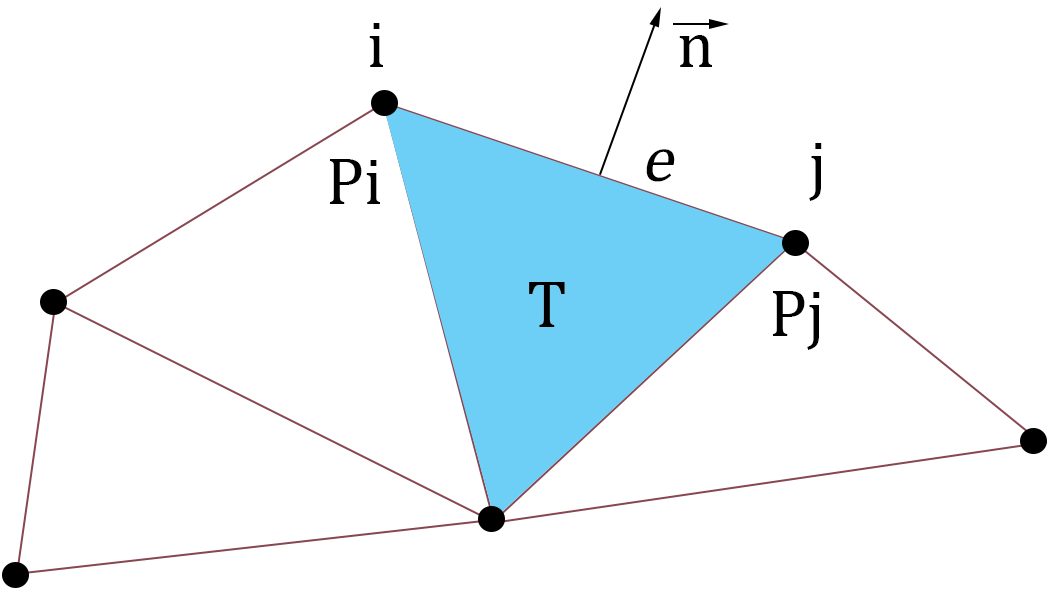
\includegraphics[height = 4cm, keepaspectratio]{graphes/bord.png}
\caption{arêtes}
\label{figure 1}
\end{center}
\end{figure}
\[
	|e|\times \vec{\text{n}}_{e}
	=
	\begin{pmatrix}
		y_{j}-y_{i} \\
		x_{i}-x_{j}
	\end{pmatrix}
\]
avec le changement de variable $x = s\times \text{Pi} + (1-s)\times \text{Pj}$,\ \ $s \in [0;1]$
\[
	\int_{e}\varphi_{i}.\vec{\text{n}}_{e}\ \partial s = |e|(\int_{0}^{1}\varphi_{i}\ \partial x ).\vec{\text{n}}_{e}
\]
avec 
\[
	\int_{0}^{1}\varphi_{i}\ \partial s  = \text{aire du triangle rectangle de coté |e| et de hauteur 1} = \frac{|e|}{2}
\]
d'où
\[
	\int_{e}\varphi_{i}.\vec{\text{n}}_{e}\ \partial s =
	|e|(\int_{0}^{1}\varphi_{i}\ \partial x ).\vec{\text{n}}_{e} =
	\frac{|e|}{2}.\vec{\text{n}}_{e} = 
	\frac{|e|^{2}}{2}
	\begin{pmatrix}
		y_{2}-y_{1} \\
		x_{1}-x_{2}
	\end{pmatrix}	
\] 
Au final
\[
	\iint_{\Omega}\bigtriangledown_{x}{\varphi_{i}} =
	\sum_{e \in \partial \text{supp}(\varphi_{i})}\ \int_{e}\varphi_{i}.\vec{\text{n}}_{e}\ \partial s =
	\sum_{e \in \partial\text{supp}(\varphi_{i})}
	\frac{|e|}{2}
	\begin{pmatrix}
		y_{2}-y_{1} \\
		x_{1}-x_{2}
	\end{pmatrix}
\]
\[
	\iint_{\Omega}\bigtriangledown_{x}{\varphi_{i}} =
	\sum_{e \in \partial \text{supp}(\varphi_{i})}
	\frac{|e|}{2}
	\begin{pmatrix}
		x_{2}-x_{1} \\
		y_{1}-y_{2}
	\end{pmatrix}
\]
Au final 
\[\boxed{f_{j} =  -\vec{e_{y}}.\sum_{e \in \partial \text{supp}(\varphi_{i})}
	\frac{|e|}{2}
	\begin{pmatrix}
		x_{2}-x_{1} \\
		y_{1}-y_{2}
	\end{pmatrix}}
\]

				

%==================================== Calcul du gradient ==================================================================================================																																							
\subsection{Calcul du Gradient}

Ce que nous voulons obtenir à l'issue de notre étude du potentiel $u$, c'est le champ magnétique $\vec{B}$, que l'on peut calculer en tout point du maillage par la même méthode numérique, que l'on a utilisé pour calculer le potentiel u.
\newline On pose donc  $\vec{B}= \bigtriangledown u$.
\\
\newline  On écrit la forme variationnelle dans $V_{h}$ (ainsi B suit une décomposition dans $V_h$, tel que $B=\sum_{i} B_{xi}\varphi_i:$

\[
\begin{aligned}
		\forall \varphi \in V_{h} , \ \int_{\Omega}B.  \varphi &= \int_{\Omega}\bigtriangledown u.\varphi  \\
		\sum_{i,j}\;  \sum_{T \in \text{Supp}(\varphi_{i})\times \text{Supp}(\varphi_{j})}B_{i}\int_{T} \varphi_i\varphi_j & =  \sum_{i}  \sum_{T \in \text{Supp}(\varphi_{i})\times \text{Supp}(\varphi_{j})} u_i \int_{T}\bigtriangledown\varphi_i\varphi_j  
\end{aligned}
\]
On peut donc réécrire l'équation précédente comme un problème linéaire sous forme matricielle  $M \times B=C \times U $

Nous pouvons écrire l'équation ci dessus sous forme matricielle, en introduisant M et C, définit de la façon suivante :
\[
		M_{ij}=\int_{T} \varphi_i.\varphi_j \ \text{appellé la matrice de masse}
\]
\[
		C_{ij}=\int_{T} \bigtriangledown\varphi_i.\varphi_j 
\]
Soit 
\[
	\boxed{B =M\up{-1}\times C \times U}
\]

On va donc comme la matrice de rigidité, remplir les matrices M et C à l'aide de matrices élémentaires. 
\\
Calculons ainsi les termes de la matrice C:
\[
\begin{aligned}
C_{ij} &= \iint_{\Omega}\bigtriangledown\varphi_i\varphi_j dx      
       = \sum_{K\in supp\varphi_j}\bigtriangledown_K\varphi_i \iint_{K} \varphi_jdx \\
	 &= \sum_{K\in supp\varphi_j}(J\up{-1}_K)^{T}(\bigtriangledown_{\hat{K}} \hat{\varphi_i})\iint_{\hat{K}}  |J_{K}| \hat{\varphi_j}\hat{dx} \\
	&= \sum_{K\in supp\varphi_j}(J\up{-1}_K)^{T}|J_K| (\bigtriangledown_{\hat{K} }\hat{\varphi_i})\iint_{\hat{K}}  \hat{\varphi_j}\hat{dx}
\end{aligned}
\]
\[\boxed{C_{ij} =  \sum_{K\in supp\varphi_j}(J\up{-1}_K)^{T}|J_K| (\bigtriangledown_{\hat{K} }\hat{\varphi_i})\iint_{\hat{K}}  \hat{\varphi_j}\hat{dx}} \]
Calculons une matrice élémentaire de C sur un triangle K du maillage qui aura donc pour composantes (si on se place selon la composante x du gradient ) 

\[
|J_K| \times
\begin{pmatrix}
   	\bigtriangledown_{\hat{K} }{\varphi_1}_{|x}\iint_{\hat{K}}  \hat{\varphi_1}&\bigtriangledown_{K}{\varphi_1}_{|x}\iint_{\hat{K} } \hat{\varphi_2} &\bigtriangledown_{K}{\varphi_1}_{|x}\iint_{\hat{K} } \hat{\varphi_3}\\ 
  \bigtriangledown_{K }{\varphi_2}_{|x}\iint_{\hat{K }} \hat{\varphi_1} & \bigtriangledown_{K }{\varphi_2}_{|x}\iint_{\hat{K} }\hat{\varphi_2} & \bigtriangledown_{K }{\varphi_2}_{|x}\iint_	{\hat{K} } \hat{\varphi_3} \\
  \bigtriangledown_{K }{\varphi_3}_{|x}\iint_{\hat{K} } \hat{\varphi_1}&\bigtriangledown_{K }{\varphi_3}_{|x}\iint_{\hat{K} } \hat{\varphi_2} & \bigtriangledown_{K}{\varphi_3}_{|x}\iint_{\hat{K} } \hat{\varphi_3}
\end{pmatrix} 
\]
Calculons les intégrales :


\[	
  \left\{
    \begin{aligned}
      \iint_{\hat{K}} \hat{\varphi_1}{\hat{dx}} &= \int_{0}^{1}\int_{0}^{1-{\hat{x}}_2} (1-{{\hat{x}}_1}-{{\hat{x}}_2}) \hat{dx}_1 \hat{dx}_2 &=1/6\\
      \iint_{\hat{K} } \hat{\varphi_2}\hat{dx} &= \int_{0}^{1}\int_{0}^{1-{\hat{x}}_2} {{\hat{x}}_1} \hat{dx}_1 \hat{dx}_2 =1/6\\
       \iint_{\hat{K} } \hat{\varphi_3}\hat{dx} &= \int_{0}^{1}\int_{0}^{1-{\hat{x}}_2} {{\hat{x}}_1} \hat{dx}_1 \hat{dx}_2 =1/6\\
    \end{aligned}
  \right.
\]
On a ainsi a matrice élémentaire du terme C sur un triangle K:

\[
\frac{1}{6}\times
	\begin{pmatrix}
   		\bigtriangledown_{K}{\varphi_1}_{|x} & \bigtriangledown_{K}{\varphi_1}_{|x} &  										    
   		\bigtriangledown_{K} {\varphi_1}_{|x} \\ 
    	\bigtriangledown_{K }{\varphi_2}_{|x} & \bigtriangledown_{K }{\varphi_2}_{|x} &  
    	\bigtriangledown_{K }{\varphi_2}_{|x} \\    										        
    	\bigtriangledown_{K}{\varphi_3}_{|x} & \bigtriangledown_{K}{\varphi_3}_{|x} & \bigtriangledown_{K}{\varphi_3}_{|x} \\ 
    \end{pmatrix} 
\]
Calcul de la matrice M
\[
M_{ij}=\iint_\Omega \varphi_i \varphi_j
\]
Sur un triangle K du maillage , on obtient de la même manière que précédemment 
\[
  \left.
    \begin{aligned}
		M_{ij}\up{K}=\int_0^{1}\int_0^{1-{\hat{x}}_2}|J_K|\hat{\varphi_i}(\hat{x})\hat{\varphi_j}(\hat{x})d\hat{x}\\
		=2\times\text{aire}(K)\times\int_0^{1-{\hat{x}}_2}\hat{\varphi_i}(\hat{x})\hat{\varphi_j}(\hat{x})d\hat{x}
    \end{aligned}
  \right.
\]
Il suffit donc de calculer les intégrales 
\[
	\int _0^{1}\int_0^{1-{\hat{x}}_2}\hat{\varphi_i}(\hat{x})\hat{\varphi_j}(\hat{x})d\hat{x}
\]
\\
par symétrie 
\[
	\forall i \int _0^{1}\int_0^{1-\hat{x}_{2}}\hat{\varphi_i}\up{2}= \int _0^{1} \int_0^{1-\hat{x}_{2}}\hat{x}_{2}^{2}d\hat{x}_{1}d\hat{x}_{2}=\frac{1}{12}
\]
\\%
\[
	\forall i \neq j \int _0^{1}\int_0^{1-{\hat{x}}_2}\hat{\varphi_i} \times \hat{\varphi_j}=\int _0^{1} \int_0^{1-\hat{x}_{2}}\hat{x}_{1}\hat{x}_{2}d\hat{x}_{1}d\hat{x}_{2}=\frac{1}{24}
\]
\\%
On en déduit la matrice de masse élémentaire sur un triangle de maillage 
\\%
\[
	\boxed{M\up{K}=\frac{\text{aire}(K)}{12}\times 
	\begin{pmatrix}
   		2 & 1 & 1 \\
   		1 &  2 & 1 \\
   		1 &  1 & 2
	\end{pmatrix}}
\]

%======================================== Algorithme Matlab ===============================================================================================
\subsection{Implémentation algorithmique}

Pour la résolution du problème nous utiliserons matlab avec la bibliothèque Mesh2D par Darren Engwirda pour la création du maillage 2D.
La résolution est effectué sur un maillage $5\times 5$cm avec en son centre un aimant de taille $1\times 1$cm.

\begin{figure}[h]
\begin{center}
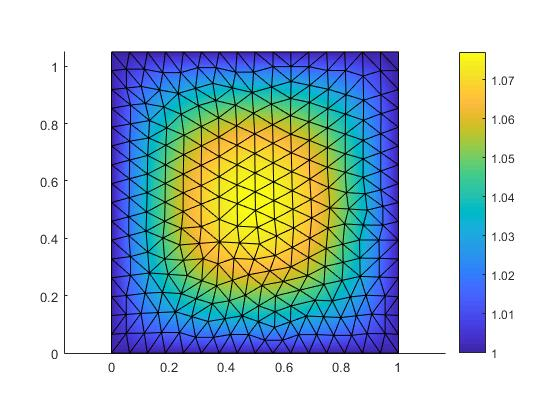
\includegraphics[height = 5cm, keepaspectratio]{graphes/sheme.jpg} 
\caption{\label{figure 3 } maillage effectué sur matlab à l'aide de mesh2D pour la résolution du problème}
\end{center}
\end{figure}
\newpage
Pour le calcul nécessaire des différentes matrice afin de résoudre le problème linéaire $A\times U = F$, les algorithmes reposent sur la méthodologie suivante :
Par exemple pour le calcul de la matrice A : 
\[
\begin{aligned}
A_{ij} = 
	\iint_{\Omega}\bigtriangledown_{x}{\varphi_{i}} \bigtriangledown_{x}{\varphi_{j}} &= 
	\sum_{T \in \text{Supp}(\varphi_{i})\times \text{Supp}(\varphi_{j})}	
	\frac{\text{aire}(T)^{2}}{4}
	\begin{pmatrix}
   		y_{3}-y_{1} &  	x_{1}-x_{3}\\
   		y_{1}-y_{2} &  x_{2}-x_{1}
	\end{pmatrix}
	^{2}
	\bigtriangledown_{\hat{x}} \hat{\varphi_{i}}
	\bigtriangledown_{\hat{x}} \hat{\varphi_{j}}
\end{aligned}
\]
Le principe consiste à ne pas recherche le support croisé des fonctions phi (ce qui donnerait une complexité trop importante) mais à boucler sur les triangles et placer dans la matrice les contributions correspondantes à chacun de leurs nœuds avec leur indices. Notamment avec l'outil matriciel $sparce$ de matlab qui permet d'exploiter en temps de calcul et d'espace mémoire le fait que la matrice A est creuse, comme pour deux fonction $\varphi_{i}$ et $\varphi_{j}$ l'intersection de leurs support se réduit à deux triangles. 
\\
\\
Ainsi pour le calcul de A chaque triangle engendre une matrice $ 3\times 3$ symétrique vu le calcul du terme $A_{ij}$ dont on place les terme dans la matrice A.
\\
\\Le principe est le même pour le terme source, pour chaque triangle appartenant au bord de l'aimant avec comme noeuds sur le bord les nœuds $\text{p}_{i}$ et  $\text{p}_{j}$ on place deux fois le même terme $\frac{|e|}{2}\begin{pmatrix}
   									0 & 1\\
								\end{pmatrix}^{T}.
								\vec{\text{n}}_{e}$ 
aux indices $\text{p}_{i}$ et  $\text{p}_{j}$ dans la matrice du terme source.
\\
\\
Et de même également pour le calcul des matrices M et C pour le gradient.		
%===============================================================================================================================										% Application à Navier Stokes  3D																															
%================================================================================================================================================================
\chapter{Application au problème de Navier-Stokes 3D}		
Après l'implantation d'une méthode pour calculer le champ magnétique en 2 dimensions , il nous est nécessaire de nous replacer dans le cas de Navier-Stokes en 3 dimensions.
\\ 
\\ 
En effet nous avons effectué l'étude précédente dans le cas d'un milieu neutre de longueur L , et de largeur H, avec les lignes de champ magnétique issue d'un aimant au milieu de l'espace. 
L'objectif est d'abord d'extraire de cet espace le champ magnétique qui se trouve dans la cuve apposée à l'aimant. 
\\
Avant toute chose, il est important de comprendre quelle configuration préalable de modélisation numérique ,  nous devons prendre pour notre cuve, car l'algorithme de calcul numérique de l'équation de Navier-Stokes 3D vers lequel nous allons devoir exporter les valeurs du champ magnétique prend les valeurs de forces magnétiques  de Laplace uniquement sous un certain format.  Nous devons donc préalablement présenter l'algorithme de calcul de l'équation de Navier-Stokes 3D sous lequel nous travaillons. 
\\
\\

%=================================

\subsection{Implémentation algorithmique}

Sous Matlab, nous avons utilisé un algorithme de résolution d'équations dérivées partielles avec la méthode 3D de différences finies :  elle consiste à discrétiser le domaine en grille et approcher les opérateurs par des différences, ce qui nous permet d’obtenir une approximation de la vitesse et la pression en chaque nœud de la grille.  
\\ \\
Le domaine $\Omega = ]0;L_x[ . ]0;L_y[.]0;L_z[$ est discrétisé par un maillage uniforme défini par les points : 
\\

\[
\left\{
\begin{array}{ccc}
  x_{ij} = (\frac{i*L_x}{N+1} ,\frac{j*L_x}{N+1}),    i,j=0,1,......,N+1\\
  y_{ij} = (\frac{i*L_y}{N+1} ,\frac{j*L_y}{N+1}),    i,j=0,1,......,N+1  \\
 z_{ij} = (\frac{i*L_z}{N+1} ,\frac{j*L_z}{N+1}),    i,j=0,1,......,N+1  
\end{array}
\right.
\]
On cherche les approximations :
\[
u_{ij}^{(1)} \approx u_1(x_{ij}) \\\\\ \text{et} \\\ u_{ij}^{(2)} \approx u_2(x_{ij}) 
\]
\\
avec $u^(1)$ et $u^(2)$ les deux composantes de la vitesse exacte $V^{~}$en 2D.
Pour discrétiser le système d'équations 4.1, nous utilisons la méthode de différences finies centrée.
On pose h= $\frac{1}{N+1}$: 
\begin{figure}[h]
	\center
	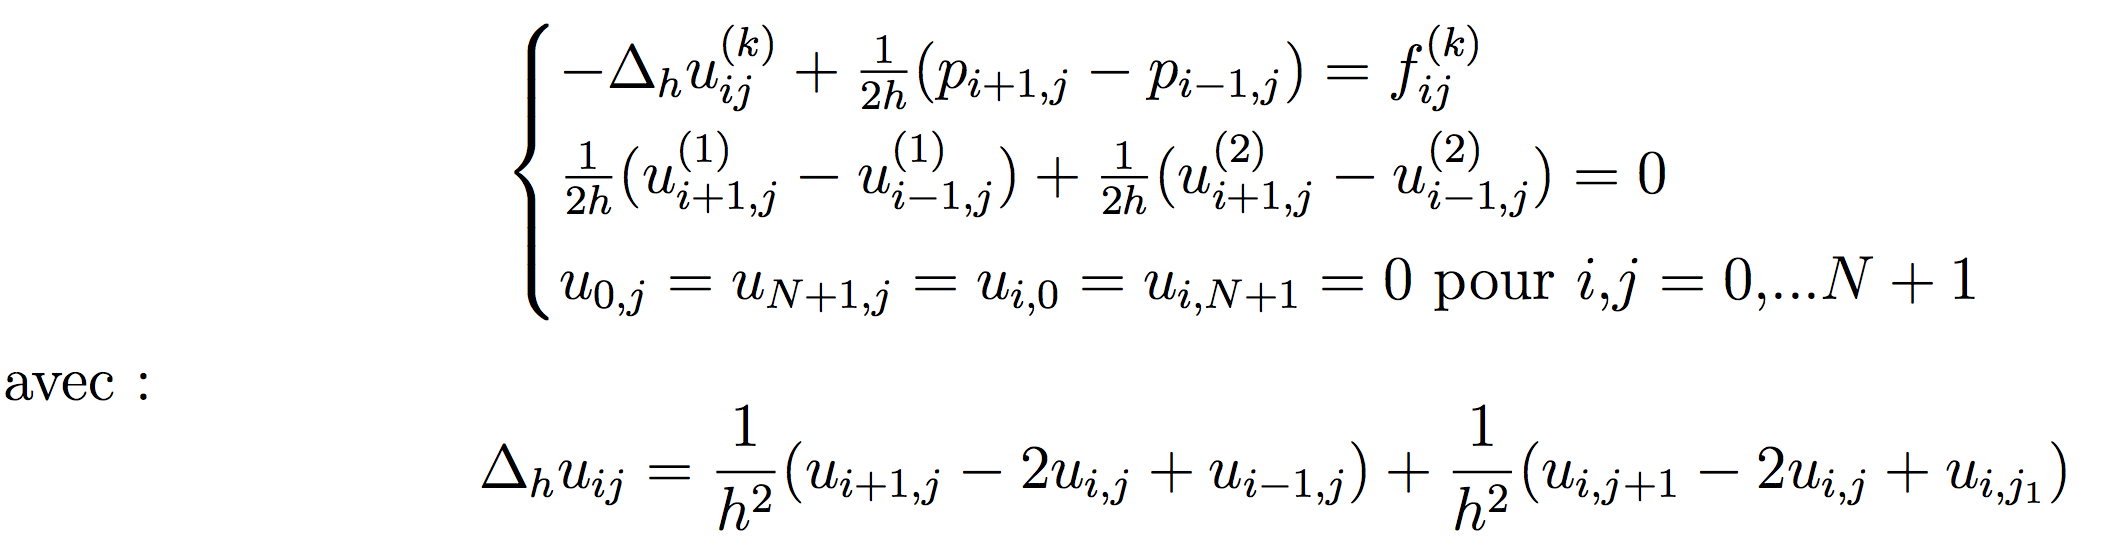
\includegraphics [height = 3.5cm, keepaspectratio]{graphes/equation1stokes.png}
\end{figure}


%Pour modéliser ce nouvel espace, nous prenons la configuration suivante :
Nous disposons de $3N^2$ équations . Les maillages sur $\vec{V}$ et P sont choisis de sorte que le nombre d'équations soit égal au nombre d'inconnues.
Le maillage 3D utilisé par l'algorithme est un maillage droit , ce qui implique que les données que l'on va exporter sont calculées et configurées sur la même base  de maillage triangulaire en 2 dimensions de l'espace de calcul. 
	\\\
\begin{figure}
\center
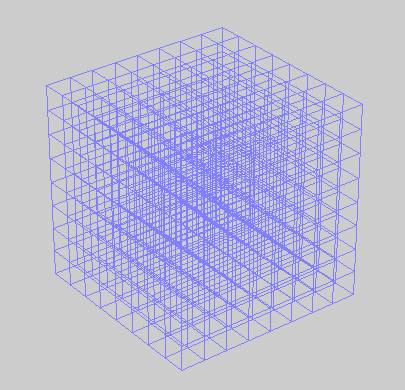
\includegraphics[height = 10cm, keepaspectratio]{graphes/maillage_droit.png}
\caption{domaines de résolution du problème}																													
\end{figure}






Nous devons adapter notre maillage précédent du calcul de la force de Laplace à l'aide des éléments finis aux besoins de l'algorithme précédent: 
\newline
\newline
tout d'abord nous devons travailler sur un maillage triangulaire droit dont les dimensions coincident avec le maillage de la base de l'espace de travail précédent. Nous prenons une largeur L , un profondeur P, et une hauteur H pour la cuve avec un nombre de points Nx*Ny pour le maillage.  Afin d'avoir un maillage qui colle à ces contraintes, nous allons utiliser la fonction delaunay de Matlab, qui prend en argument les coordonnées x et y des points de l'espace que nous allons mailler. 
\newline
ci dessous le maillage de l'espace de travail  initial sur laquelle nous allons calculer notre fonction champ magnétique:
\begin{figure}[!h]
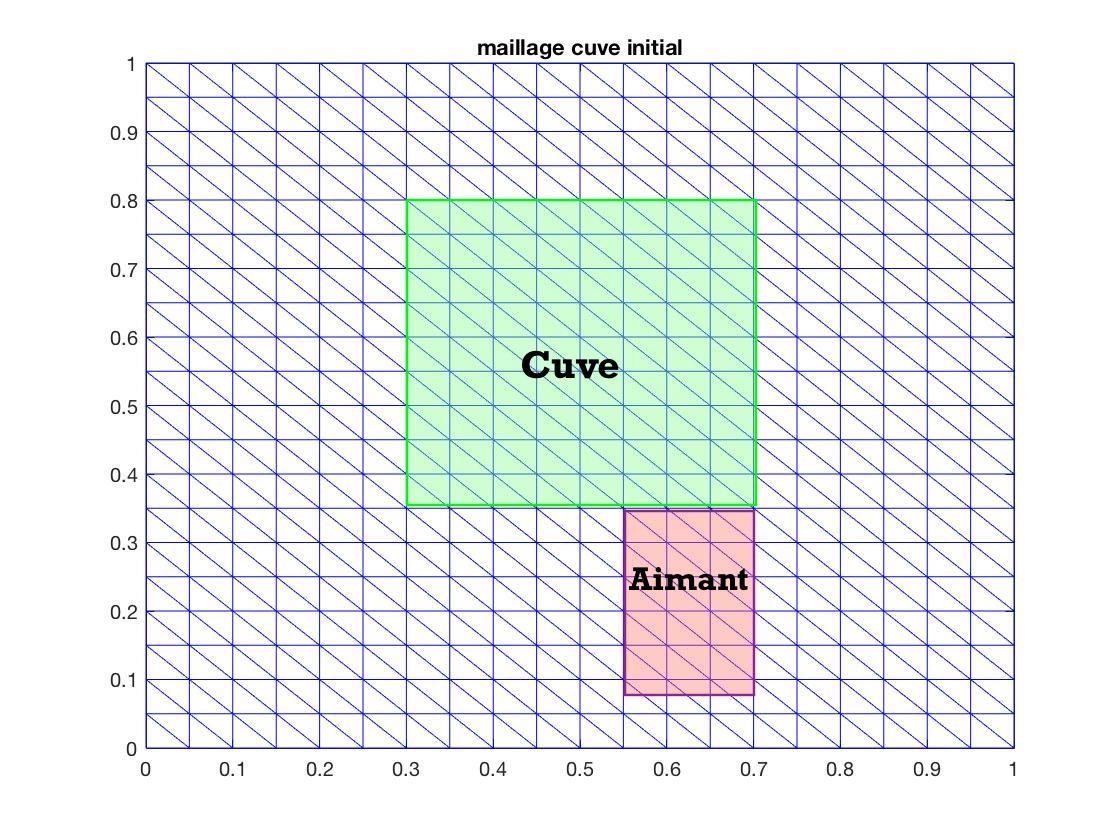
\includegraphics[height = 10cm, keepaspectratio]{graphes/Maillage_initial1.jpg}
\caption{\label{figure 3 } maillage effectué sur matlab à l'aide de mesh2D pour la résolution du problème}

\end{figure}
\newline
Néanmoins nous devons auparavant nous replacer dans le contexte initial : le maillage précédent ne servirait qu'à calculer le champ magnétique sur tout l'espace avec  l'aimant au milieu de l'espace et avec approximation de quasi nullité de la fonction aux bords de l'espace de travail. 
\\
Or ce qui nous intéresse est le calcul du champ magnétique uniquement dans la cuve, qui est accolée à l'aimant. Il y a donc un travail préalable de redécoupage de l'espace après calcul du champ magnétique en dimensionnant l'aimant selon des coordonnées particulières. 
\newline


L'objectif est d'extraire les noeuds, triangles et valeurs de champ magnétique associés à cette espace. Il faut donc dans les programmes précédents inclure des commandes supplémentaires afin d'assigner à chaque objet précédent un nouvel attribut entre  $\{0,1,2\}$ qui détermine si l'on est soit dans l'aimant , soit dans la cuve, soit dans l'espace environnant (notamment avec l'attribut fnum, utilisé dans le calcul du second membre des éléments finis). 
\newline
Maintenant  notre objectif est de pouvoir adapter les données extraites à l'algorithme de Stokes 3D. Le premier obstacle est de réindexer le numéro des triangles pour qu'il y ait une bonne consistance des données lorsque l'algorithme va les utiliser: il faut renuméroter les triangles dans l'ordre. 
\newline 
\newline
Un autre obstacle est la structure de calcul sur les cubes du champ de vitesse par l'algorithme qui se base sur l'équation de Navier Stokes: 
\newline
l'algorithme de Navier Stokes calcule le champ de vitesse dans le maillage cubique de l'espace, avec par cellule de calcul de 8 cubes , une connectivité de 27 points répartis avec une indexation particulière qu'il faudra prendre en compte lors du transfert des résultats du champ magnétique vers cette algo. On notera la présence par arête de 3 points , et non pas 2 (un de plus au milieu) : en effet l'algorithme utilisé pour résoudre numérique de Navier Stokes est  la méthode de différences finies centrée.
\newline
Cette algorithme prend en argument comme vu précedemment la matrice de rigidité A  , et le second membre se rapportant à la force électromagnétique de Laplace. Lorsque l'on veut programmer le second membre dans l'algorithme à partir des coordonnées f(x,y) dans l'espace 3D pour le mettre au format vectoriel demander par l'algorithme, on remplit le second membre selon la table de connectivité ci dessous.
\begin{figure}[!h]
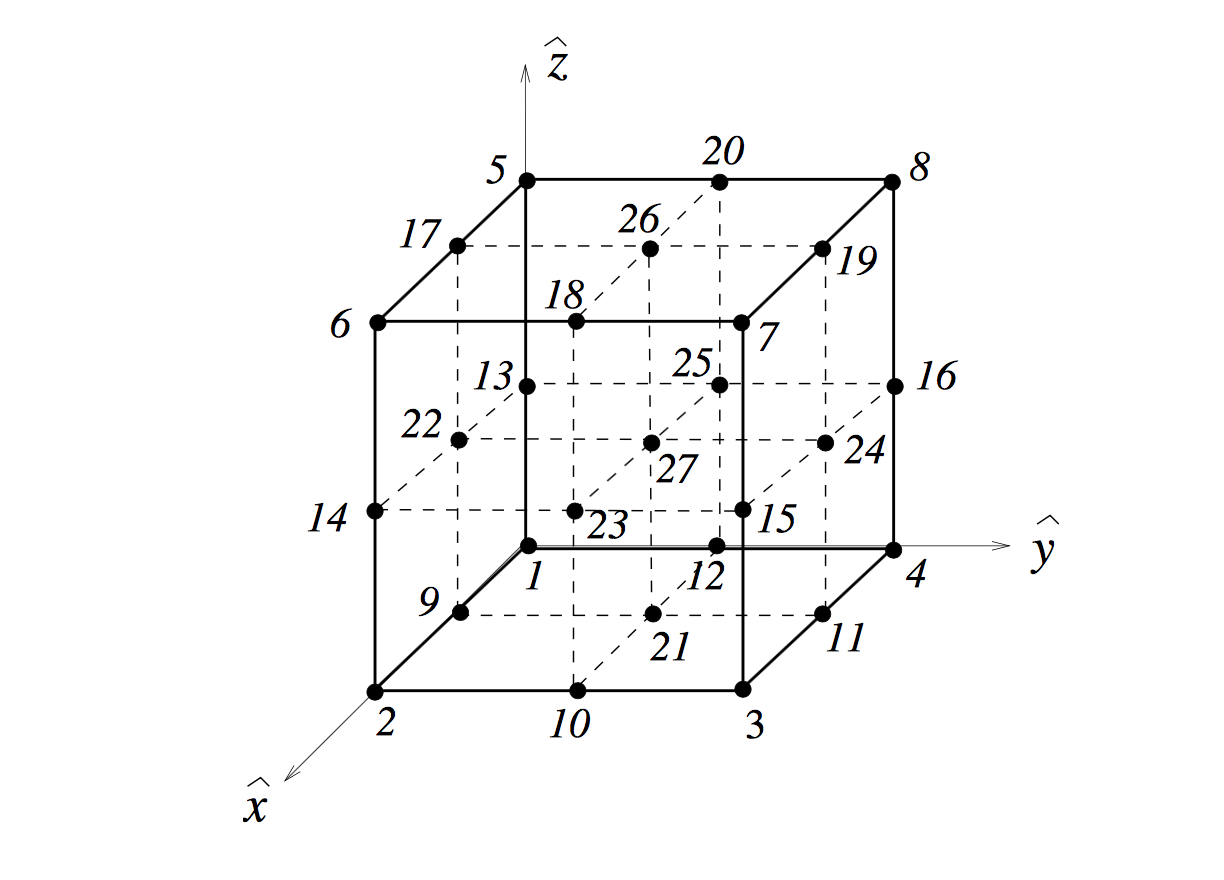
\includegraphics[height = 10cm, keepaspectratio]{graphes/table_de_connectivite.png} 
\caption{\label{figure 3 } table de connectivité pour le remplissage du second membre dans l'algorithme de résolution de l'équation de Navier Stokes}
\end{figure}
\newline
\newline
\newline
\newline
\newline
\newline
\newline
\newline
\newline
\newline
\newline
\newline
\newline
\newline
\newline
\newline
Prenons par exemple les 9 premiers termes de la fonction force de Laplace au niveau $z=0$ à partir de l'origine de ce plan dans le maillage de la cuve. Schématiquement si l'on se limite à la portion $[0;2/N_x].[0;2/N_y]$, on remplit le vecteur $\vec{f_z}$
\\
\[
\vec{f_z}=
\left(
\begin{array}{ccc}
  f_z(0,0) & f_z(1/N_x,0) & f_z(2/N_x ,0)\\
  f_z(0,1/N_y) & f_z(1/N_x,1/N_y) & f_z(2/N_x ,1/N_y) \\
  f_z(0,2/N_y) &  f_z(1/N_x,2/N_y) & f_z(2/N_x,2/N_y )
\end{array}
\right) \overset{\text{selon table de connectivité}}{\Longrightarrow}
\left(
\begin{array}{ccc}
  f_z(0,0)     \\
  f_z(2/N_x ,0)      \\
      f_z(2/N_x,2/N_y )  \\
     f_z(0,2/N_y)\\ 
  ...\\
  f_z(1/N_x,0)\\
   f_z(2/N_x ,1/N_y)\\
   f_z(1/N_x,2/N_y) \\
   f_z(0,1/N_y)\\
   ... \\
    f_z(1/N_x,1/N_y)
\end{array}
\right)
\]
\\
\\



%==========================================================================================================================================================
%														Annexe
%==========================================================================================================================================================

\begin{appendix}
\chapter{Calcul de la matrice de rigidité}
\label{annexe_1}

La matrice Jacobienne de la transformation est définie par
\[	
J =
\begin{pmatrix}
  \frac{\partial\varphi_{1}}{\partial \hat{x}_{1}} & \frac{\partial\varphi_{2}}{\partial \hat{x}_{2}}  & \frac{\partial\varphi_{3}}{\partial \hat{x}_{1}}\\ 
  \frac{\partial\varphi_{1}}{\partial \hat{x}_{2}} & \frac{\partial \varphi_{2}}{\partial \hat{x}_{2}} & \frac{\partial\varphi_{3}}{\partial \hat{x}_{2}} 
\end{pmatrix} 
\times
\begin{pmatrix}
   x_{1} &  y_{1} \\
   x_{2} &  y_{2} \\
   x_{3} &  y_{3}
\end{pmatrix}
\]
\[
\frac{\partial \hat{\varphi}}{\partial \hat{x}_{1}}(\hat{x}) = 
\frac{\partial}{\partial \hat{x}_{1}}(\varphi(F(\hat{x})) = 
\frac{\partial \varphi}{\partial x_{1}}(x) \frac{\partial F_{1}}{\partial \hat{x}_{1}}(\hat{x}) +
\frac{\partial \varphi}{\partial x_{2}}(x) \frac{\partial F_{2}}{\partial \hat{x}_{1}}(\hat{x})
\]

Donc
\[ \bigtriangledown_{\hat{x}} \hat{\varphi} = 
\begin{pmatrix}
   \frac{\partial F_{1}}{\partial \hat{x}_{1}} & \frac{\partial F_{2}}{\partial \hat{x}_{2}}\\
\end{pmatrix}
\times 
\begin{pmatrix}
   \frac{\partial \varphi}{\partial x_{1}}(x) \\
   \frac{\partial\varphi}{\partial x_{2}}(x)
\end{pmatrix} = 
J^{T} \times \bigtriangledown_{x} \varphi \]

Calculons $\bigtriangledown_{\hat{x}} \hat{\varphi}$ sur le triangle de référence $\hat{T}$ :
\[
\left\{
\begin{array}{ccc} 
	\begin{aligned}
		\hat{\varphi}_{1} &= -\hat{x}_{1}+1-\hat{x}_{2} \\  %\qquad 	
		\hat{\varphi}_{2} &= \hat{x}_{1}                \\  %\qquad 
		\hat{\varphi}_{3} &= \hat{x}_{2}
	\end{aligned}
\end{array}
\right.
\]
En effet $\hat{\varphi}_{1}$ vaut 1 sur le sommet 1 et 0 sur les autres sommets (Figure 3).
Ainsi
\[ \bigtriangledown_{\hat{x}} \hat{\varphi}_{1} = 
\begin{pmatrix}
   -1 \\
   -1
\end{pmatrix}
\qquad
\bigtriangledown_{\hat{x}} \hat{\varphi}_{2} = 
\begin{pmatrix}
   -1 \\
   -1
\end{pmatrix}
\qquad
\bigtriangledown_{\hat{x}} \hat{\varphi}_{1} = 
\begin{pmatrix}
   -1 \\
   -1
\end{pmatrix}
\]
et donc
\[
\bigtriangledown_{\hat{x}} \hat{\varphi}(\hat{x}) = 
\begin{pmatrix}
   -1 & 1 & 0 \\
   -1 & 0 & 1 
\end{pmatrix}
\]
\[	
J =
\begin{pmatrix}
   -1 & 1 & 0 \\
   -1 & 0 & 1 
\end{pmatrix}
\times
\begin{pmatrix}
   x_{1} &  y_{1} \\
   x_{2} &  y_{2} \\
   x_{3} &  y_{3}
\end{pmatrix} =
\begin{pmatrix}
   x_{2}-x_{1} &  y_{2}-y_{1} \\
   x_{3}-x_{1} &  y_{3}-y_{1}
\end{pmatrix}
\]
Finalement,
\[
\begin{vmatrix}
   J
\end{vmatrix}
= (x_{2}-x_{1})\times (y_{3}-y_{1})-(x_{3}-x_{1})\times(y_{2}-y_{1})= 2\times\text{Aire}(T)
\]
où $|J|$ est le déterminant de la matrice $J$
et ainsi
\[ \bigtriangledown_{x} \varphi =  (J^{-1})^{T} \times \bigtriangledown_{\hat{x}} \hat{\varphi} \]
avec
\[
J^{-1} =  \frac{1}{|J|}
\begin{pmatrix}
   J_{22} & -J_{12} \\
   -J_{21} & J_{11}
\end{pmatrix}
\]
d'où
\[
*\begin{aligned}
	(J^{-1})^{T} 
	&=  	
	\frac{1}{|J|}
	\begin{pmatrix}
   		J_{22} & -J_{21} \\
   		-J_{12} & J_{11}	
	\end{pmatrix} \\
	&=
	\frac{1}{2\times \text{aire}(T)}
	\begin{pmatrix}
   		J_{22} & -J_{21} \\
   		-J_{12} & J_{11}	
	\end{pmatrix} 
	\end{aligned}
\]

Et le calcul du terme $A_{ij}$ de la matrice de rigidité, on obtient ainsi avec le changement de variable vers le triangle de référence.
\[
\begin{aligned}
	\text{A}_{ij} 
	&=
	\sum_{T \in \text{Supp}(\varphi_{i})\times \text{Supp}(\varphi_{j})} 
	\iint_{(i,j) \in T}\bigtriangledown_{x}{\varphi_{i}} \bigtriangledown_{x}{\varphi_{j}} \\
	&=
	\sum_{T \in \text{Supp}(\varphi_{i})\times \text{Supp}(\varphi_{j})}
	\iint_{(i,j) \in T} (J^{-1})^{T}|J|(J^{-1})^{T}|J|
	\times
	\bigtriangledown_{\hat{x}} \hat{\varphi_{i}}
	\times
	\bigtriangledown_{\hat{x}} \hat{\varphi_{j}} \\
	&=
	\sum_{T \in \text{Supp}(\varphi_{i})\times \text{Supp}(\varphi_{j})}	
	\frac{\text{aire}(T)^{2}}{4}
	\begin{pmatrix}
   		y_{3}-y_{1} &  	x_{1}-x_{3}\\
   		y_{1}-y_{2} &  x_{2}-x_{1}
	\end{pmatrix}
	^{2}
	\bigtriangledown_{\hat{x}} \hat{\varphi_{i}}
	\bigtriangledown_{\hat{x}} \hat{\varphi_{j}}
\end{aligned}
\]

\iffalse
%==========================================================================================================================================================	
\chapter{Démonstration de l'existence d'une solution u}
%==========================================================================================================================================================
\label{Démonstration 1}
On a : 
\[
\left \{
\begin{array}{ccc}
  \Div\vec{B} = 0   &   \\
  \vec{B} = \mu_{0}\times(\vec{grad} +\vec{M}) \\
  \vec{M_{0} } \ sur \  \Omega_{i}  \ et \ \vec{0}  \ sur \  \Omega_{e}
\end{array}
\right .
 \iff \ \left\{\begin{array}{cc} -\Delta u= -div(\vec{M})=0 \ sur\ \Omega \\ \\u \ = \ 0 \ sur \ \partial \Omega \end{array}\right.
\]
\\
donc au sens des distributions , $\forall \varphi \in D(\Omega)$ 
\[
\begin{aligned}
<-\Delta u,\varphi> &=  0 \\
\iff \sum_{k=1}^{3} <  \frac{\partial u}{\partial x_{k}}, \frac{\partial \varphi}{\partial x_{k}}> &= 0
\end{aligned}
\]
\\
Or u $\in H^{1}_{0}(\Omega)$ donc $ \frac{\partial u}{\partial x_k} \in L^{2}(\Omega)$
\\
donc $<  \frac{\partial u}{\partial x_k}, \frac{\partial \varphi}{\partial x_k}>=\int_{\Omega} \frac{\partial u}{\partial x_k} \times \frac{\partial \varphi}{\partial x_k}\, \mathrm{d}x $
\\
donc le probleme peut s'établir ainsi: $<\bigtriangledown u ,\bigtriangledown \varphi>_{L^{2}(\Omega) }= 0 ,\ \forall \varphi \in D(\Omega) $
\\
Or on sait que l'ensemble $\Omega$ est bornée dans au moins une direction 
\\
donc on peut écrire $< u,\varphi>_{H^{0}_{1}(\Omega)}=0 \ \forall \varphi \in D(\Omega) $
\\
 0 est une forme lineaire continue pour n'importe quelle espace vectoriel 
 \\ donc d'apres le théorème de représentation de Riesz, dans $H^{0}_{1}(\Omega)$,
\\
$\exists ! u_{0} \in H^{0}_{1}(\Omega)$ telle que $<u_{0},v>_{H^{0}_{1}(\Omega)}=0,\ \forall v\in {H^{0}_{1}(\Omega)} $

Pour trouver le champ magnétique, on appliquer les équations fondamentales de la magnétostatique. L'équation de Maxwell nous donne 
\[
\begin{aligned}
\Rot{\vec{H}} &= \vec {0} \\
\Div{\vec{B}} &= 0
\end{aligned}
\]

Le domaine étant simplement connexe, $\vec{H}$ dérive d'un potentiel U.
\[\vec{H}= \Grad{\vec{U}}\]
\[\vec{B} = \mu_{0}\times(\vec{\Grad{U}}+\vec{M})\]

Au sens des distributions pour toute fonction $\varphi\ $ dans $D(\Omega)$
\[<\Div\vec{B},\varphi> =  <-\vec{B},\vec{\Grad{\varphi}}>\]
On suppose $\vec{B} \in L^{3}_{1}(\Omega)$
\[<\Div\vec{B},\varphi> =  -\int_{\Omega}\vec{B}. \vec{\Grad{\varphi}}\]
\[<\Div\vec{B},\varphi> =  -\int_{\Omega}\mu_{0}(\vec{\Grad{U}}+\vec{M}) .{\Grad{\varphi}} = 0\]
Ainsi
\[\int_{\Omega}(\vec{\Grad{U}}+\vec{M}) . \vec{\Grad{\varphi}} = 0\]
Et comme $\vec{M}$ est nul en dehors du domaine $\Omega_{\text{int}}$ de l'aimant, on obtient (1)
\fi



\iffalse
%==========================================================================================================================================================
\chapter{Démonstration équation (1)}
%==========================================================================================================================================================
\label{Démonstration 2}	
	Pour trouver le champ magnétique, on appliquer les équations fondamentales de la magnétostatique. L'équation de Maxwell nous donne 
	\[
		\left\{
		\begin{array}{ccc}
			\begin{aligned}
				\Rot{\vec{H}} &= \vec {0} \\
				\Div{\vec{B}} &= 0
			\end{aligned}
		\end{array}
		\right.
	\]

	Le domaine étant simplement connexe, $\vec{H}$ dérive d'un potentiel $u$	.
	\[
		\left\{
		\begin{array}{ccc}		
		\begin{aligned}
			\vec{H} &= \Grad{\vec{u}} \\
			\vec{B} &= \mu_{0}\times(\vec{\Grad{u}}+\vec{M})
		\end{aligned}
		\end{array}
		\right.
	\]

	Au sens des distributions pour toute fonction $\varphi\ $  dans $D(\Omega)$	
	\[<\Div\vec{B},\varphi> \ = \ <-\vec{B},\vec{\Grad{\varphi}}>\]
	On suppose $\vec{B} \in L^{3}_{1}(\Omega)$
	\[<\Div\vec{B},\varphi> \ = \  -\int_{\Omega}\vec{B}. \vec{\Grad{\varphi}}\]
	\[<\Div\vec{B},\varphi> \ = \ -\int_{\Omega}\mu_{0}(\vec{\Grad{u}}+\vec{M}) .{\Grad{\varphi}} = 0\]
	Ainsi
	\[\int_{\Omega}(\vec{\Grad{u}}+\vec{M}) . \vec{\Grad{\varphi}} = 0\]
	Et comme $\vec{M}$ est nul en dehors du domaine $\Omega_{\text{int}}$ de l'aimant, on obtient (1)
	%je rentre l'equation on pourra y faire appel plus tard avec \ref{E}
	\[
		\forall \varphi\ \in \Omega, \ \int_{\Omega}\vec{\Grad{u}}.\vec{\Grad{\varphi}} = -\vec{M_{0}}. \int_{\Omega_{int}}\vec{\Grad{\varphi}}
	\]
\fi

\end{appendix}
\end{onehalfspace}

\newpage
\Large \bf Bibliographie

\mdseries  "Introduction à l'analyse numérique"(1998), de Jacque Rappaz et Marco Picasso, publié par les Presses polytechniques et universitaires romandes.
\\
\\
"Méthode des éléments finis : élasticité plane" par Yves Dabard, Institut Universitaire de Technologie du Mans Département Génie Mécanique et Productique
, http://iut.univ-lemans.fr/ydlogi/index.html, 24 mars 2006 – 29 mars 2011
%
%" par un écoulement stationnaire de fluide à faible Reynolds", par Ismail Mebsout et Oumaima Hammami, 2017,  Institut ´ Elie Cartan de Lorraine.
%
\\
\\
\mdseries "Analyse numérique des équations de Navier-Stokes",de Jean-François Scheid,  Cours de Master 2 Mathématiques (Recherche) - Université de Lorraine, Nancy.
\\
\\
\mdseries "Projet de deuxième Année : Génération de maillages 2D avec Matlab" de Jean-Philippe LEBOUCHER Benjamin PACCOU avec comme chef de Projet Jonas KOKO, Institut
Supérieur d’ Informatique, de Modélisation et de leurs Applications
\bibliographystyle{plain}
\bibliography{bibli}




 



\end{document}








